% Options for packages loaded elsewhere
\PassOptionsToPackage{unicode}{hyperref}
\PassOptionsToPackage{hyphens}{url}
%
\documentclass[
]{book}
\usepackage{amsmath,amssymb}
\usepackage{iftex}
\ifPDFTeX
  \usepackage[T1]{fontenc}
  \usepackage[utf8]{inputenc}
  \usepackage{textcomp} % provide euro and other symbols
\else % if luatex or xetex
  \usepackage{unicode-math} % this also loads fontspec
  \defaultfontfeatures{Scale=MatchLowercase}
  \defaultfontfeatures[\rmfamily]{Ligatures=TeX,Scale=1}
\fi
\usepackage{lmodern}
\ifPDFTeX\else
  % xetex/luatex font selection
\fi
% Use upquote if available, for straight quotes in verbatim environments
\IfFileExists{upquote.sty}{\usepackage{upquote}}{}
\IfFileExists{microtype.sty}{% use microtype if available
  \usepackage[]{microtype}
  \UseMicrotypeSet[protrusion]{basicmath} % disable protrusion for tt fonts
}{}
\makeatletter
\@ifundefined{KOMAClassName}{% if non-KOMA class
  \IfFileExists{parskip.sty}{%
    \usepackage{parskip}
  }{% else
    \setlength{\parindent}{0pt}
    \setlength{\parskip}{6pt plus 2pt minus 1pt}}
}{% if KOMA class
  \KOMAoptions{parskip=half}}
\makeatother
\usepackage{xcolor}
\usepackage{color}
\usepackage{fancyvrb}
\newcommand{\VerbBar}{|}
\newcommand{\VERB}{\Verb[commandchars=\\\{\}]}
\DefineVerbatimEnvironment{Highlighting}{Verbatim}{commandchars=\\\{\}}
% Add ',fontsize=\small' for more characters per line
\usepackage{framed}
\definecolor{shadecolor}{RGB}{248,248,248}
\newenvironment{Shaded}{\begin{snugshade}}{\end{snugshade}}
\newcommand{\AlertTok}[1]{\textcolor[rgb]{0.94,0.16,0.16}{#1}}
\newcommand{\AnnotationTok}[1]{\textcolor[rgb]{0.56,0.35,0.01}{\textbf{\textit{#1}}}}
\newcommand{\AttributeTok}[1]{\textcolor[rgb]{0.13,0.29,0.53}{#1}}
\newcommand{\BaseNTok}[1]{\textcolor[rgb]{0.00,0.00,0.81}{#1}}
\newcommand{\BuiltInTok}[1]{#1}
\newcommand{\CharTok}[1]{\textcolor[rgb]{0.31,0.60,0.02}{#1}}
\newcommand{\CommentTok}[1]{\textcolor[rgb]{0.56,0.35,0.01}{\textit{#1}}}
\newcommand{\CommentVarTok}[1]{\textcolor[rgb]{0.56,0.35,0.01}{\textbf{\textit{#1}}}}
\newcommand{\ConstantTok}[1]{\textcolor[rgb]{0.56,0.35,0.01}{#1}}
\newcommand{\ControlFlowTok}[1]{\textcolor[rgb]{0.13,0.29,0.53}{\textbf{#1}}}
\newcommand{\DataTypeTok}[1]{\textcolor[rgb]{0.13,0.29,0.53}{#1}}
\newcommand{\DecValTok}[1]{\textcolor[rgb]{0.00,0.00,0.81}{#1}}
\newcommand{\DocumentationTok}[1]{\textcolor[rgb]{0.56,0.35,0.01}{\textbf{\textit{#1}}}}
\newcommand{\ErrorTok}[1]{\textcolor[rgb]{0.64,0.00,0.00}{\textbf{#1}}}
\newcommand{\ExtensionTok}[1]{#1}
\newcommand{\FloatTok}[1]{\textcolor[rgb]{0.00,0.00,0.81}{#1}}
\newcommand{\FunctionTok}[1]{\textcolor[rgb]{0.13,0.29,0.53}{\textbf{#1}}}
\newcommand{\ImportTok}[1]{#1}
\newcommand{\InformationTok}[1]{\textcolor[rgb]{0.56,0.35,0.01}{\textbf{\textit{#1}}}}
\newcommand{\KeywordTok}[1]{\textcolor[rgb]{0.13,0.29,0.53}{\textbf{#1}}}
\newcommand{\NormalTok}[1]{#1}
\newcommand{\OperatorTok}[1]{\textcolor[rgb]{0.81,0.36,0.00}{\textbf{#1}}}
\newcommand{\OtherTok}[1]{\textcolor[rgb]{0.56,0.35,0.01}{#1}}
\newcommand{\PreprocessorTok}[1]{\textcolor[rgb]{0.56,0.35,0.01}{\textit{#1}}}
\newcommand{\RegionMarkerTok}[1]{#1}
\newcommand{\SpecialCharTok}[1]{\textcolor[rgb]{0.81,0.36,0.00}{\textbf{#1}}}
\newcommand{\SpecialStringTok}[1]{\textcolor[rgb]{0.31,0.60,0.02}{#1}}
\newcommand{\StringTok}[1]{\textcolor[rgb]{0.31,0.60,0.02}{#1}}
\newcommand{\VariableTok}[1]{\textcolor[rgb]{0.00,0.00,0.00}{#1}}
\newcommand{\VerbatimStringTok}[1]{\textcolor[rgb]{0.31,0.60,0.02}{#1}}
\newcommand{\WarningTok}[1]{\textcolor[rgb]{0.56,0.35,0.01}{\textbf{\textit{#1}}}}
\usepackage{longtable,booktabs,array}
\usepackage{calc} % for calculating minipage widths
% Correct order of tables after \paragraph or \subparagraph
\usepackage{etoolbox}
\makeatletter
\patchcmd\longtable{\par}{\if@noskipsec\mbox{}\fi\par}{}{}
\makeatother
% Allow footnotes in longtable head/foot
\IfFileExists{footnotehyper.sty}{\usepackage{footnotehyper}}{\usepackage{footnote}}
\makesavenoteenv{longtable}
\usepackage{graphicx}
\makeatletter
\def\maxwidth{\ifdim\Gin@nat@width>\linewidth\linewidth\else\Gin@nat@width\fi}
\def\maxheight{\ifdim\Gin@nat@height>\textheight\textheight\else\Gin@nat@height\fi}
\makeatother
% Scale images if necessary, so that they will not overflow the page
% margins by default, and it is still possible to overwrite the defaults
% using explicit options in \includegraphics[width, height, ...]{}
\setkeys{Gin}{width=\maxwidth,height=\maxheight,keepaspectratio}
% Set default figure placement to htbp
\makeatletter
\def\fps@figure{htbp}
\makeatother
\usepackage{svg}
\setlength{\emergencystretch}{3em} % prevent overfull lines
\providecommand{\tightlist}{%
  \setlength{\itemsep}{0pt}\setlength{\parskip}{0pt}}
\setcounter{secnumdepth}{5}
\usepackage{booktabs}
\ifLuaTeX
  \usepackage{selnolig}  % disable illegal ligatures
\fi
\usepackage[]{natbib}
\bibliographystyle{plainnat}
\IfFileExists{bookmark.sty}{\usepackage{bookmark}}{\usepackage{hyperref}}
\IfFileExists{xurl.sty}{\usepackage{xurl}}{} % add URL line breaks if available
\urlstyle{same}
\hypersetup{
  pdftitle={Sistemas de Controle II (EL180)},
  pdfauthor={Rafael Suzuki Bayma},
  hidelinks,
  pdfcreator={LaTeX via pandoc}}

\title{Sistemas de Controle II (EL180)}
\author{Rafael Suzuki Bayma}
\date{2024-02-05}

\begin{document}
\maketitle

{
\setcounter{tocdepth}{1}
\tableofcontents
}
\hypertarget{apresentauxe7uxe3o}{%
\chapter{Apresentação}\label{apresentauxe7uxe3o}}

Curso de Sistemas de Controle II - Faculdade de Engenharia Elétrica, Campus Tucuruí.

Versão: 2024.2

\hypertarget{objetivos}{%
\section{Objetivos}\label{objetivos}}

Objetivo principal do curso é introduzir técnicas de modelagem, análise e projeto de sistemas de controle usando duas abordagens principais: espaço de estados e modelos de sinais e sistemas digitaisl.

\textbf{Carga horária:} 60 horas

O curso é predominantemente teórico com aplicações computacionais. Aplicações práticas em laboratório poderão ocorrer mediante disponibilidade de equipamento.

\textbf{Pré-requisitos:} Análise de Sistemas Lineares, Sistemas de Controle I.

\textbf{Recomendado:} boa compreensão de equações diferenciais, sinais e sistemas, mecânica clássica, Circuitos Elétricos I, amplificadores operacionais, Python simbólico e numérico, linguagem R (apenas para gerar trabalhos de melhor qualidade).

\hypertarget{avaliauxe7uxe3o}{%
\section{\texorpdfstring{\textbf{Avaliação:}}{Avaliação:}}\label{avaliauxe7uxe3o}}

Estimativa de 2 trabalhos divididos em 2 partes cada.

Trabalho 1 - espaço de estados. Parte 1: exame escrito com resolução de problemas básicos de baixa ordem (3a no máximo); trabalho presencial realizado em sala, individual, com consulta. Parte 2: projeto computacional resolvido em Python de um problema mais complexo, com auxílio das bibliotecas relevantes e simulação. Objetivo é fazer o projeto, simular e analisar o resultado.

Trabalho 2 - sistemas digitais. Partes seguindo o mesmo roteiro do trabalho 1, exceto agora sobre sistemas digitais.

Trabalho final - opcional, versando sobre toda a matéria. Destinado apenas aqueles que não alcançaram média ou que necessitarem de 2a chamada.

A parte computacional deve ser feita toda em Python. Os projetos devem ser entregues no formato de um relatório/dashboard em arquivo PDF ou HTML contendo os resultados e a análise. Outros formatos não serão aceitos por questões de organização e portabilidade.

Uma correção dos erros em cada trabalho poderá ser apresentada, caso autorizada, com uma penalidade na pontuação final (a definir em cada avaliação). Válido apenas aos alunos que fizeram a primeira entrega. Vedado participar da correção ao aluno que não entregou o trabalho.

A nota final é a média simples das duas maiores notas.

\hypertarget{introduuxe7uxe3o-uxe0s-tuxe9cnicas-de-espauxe7o-de-estados.}{%
\chapter{Introdução às técnicas de espaço de estados.}\label{introduuxe7uxe3o-uxe0s-tuxe9cnicas-de-espauxe7o-de-estados.}}

Os métodos de espaço de estados são importantes técnicas usadas em Engenharia de Controle para análise e projeto de sistemas. Eles são complementares às técnicas no domínio da frequência (função de transferência) e compreendem o que alguns autores chamam de ``controle moderno''.

Neste capítulo introduzimos algumas noções básicas sobre o assunto.

\hypertarget{o-que-uxe9-espauxe7o-de-estados}{%
\section{O que é espaço de estados?}\label{o-que-uxe9-espauxe7o-de-estados}}

Um modelo de espaço de estados para um sistema linear invariante no tempo (SLIT) é um conjunto de equações diferenciais ordinárias simultâneas de 1a ordem. Por exemplo:

\begin{aligned}
  \dot{x}_1 &= 2x_1-x_2+u\\
  \dot{x}_2 &= -x1
\end{aligned}

onde \(u\) é o sinal de entrada e os sinais \(x_1\) e \(x_2\) são chamados de estados do sistema. As duas primeiras equações são chamadas de equações de estado do sistema.

À equação de estados juntamos a equação de saída do sistema
\[
  y = 3x_1+4x_2 
\]
que descreve o sinal de saída \(y\) em função dos estados.

Isso é um pouco diferente do que você aprendeu em Controle I e ASL, onde os sistemas são representados por uma única EDO de ordem elevada, que contém apenas um sinal de entrada e um sinal de saída.

Em uma equação de estados temos várias equações diferenciais simultâneas em múltiplos sinais (funções do tempo) \(x_1\), \(x_2\), etc.

O número \(n\) de estados deve ser igual ao número de equações de estado. \(n\) é equivalente a ordem do sistema. Veremos depois que isso equivale a ordem da função de transferência do sistema.

Uma equação de estados substitui uma EDO de ordem \(n\) por \(n\) equações de ordem 1. Note entretanto que não conseguimos resolver essas equações de forma independente, devido à interdependência delas.

A representação de estados é uma forma alternativa de modelar matematicamente de um sistema. Ela não exclui a representação do sistema por função de transferência.

Observação:

\begin{aligned}
    \frac{dx(t)}{dt} &= \dot{x}(t) =  \dot{x}\\
    \frac{d^2x(t)}{dt^2} &= \ddot{x}(t) = \ddot{x}
\end{aligned}

\hypertarget{o-que-uxe9-estado}{%
\section{O que é estado?}\label{o-que-uxe9-estado}}

Matematicamente, os estados funções do tempo intermediárias que precisam ser resolvidas para obtermos o sinal de interesse do sistema, isto é, o sinal de saída.

Fisicamente, os estados denotam grandezas físicas importantes, que determinam como o sistema evolui, mas não são necessariamente mensuráveis.

Um bom exemplo é o modelo físico de um gás. Em termodinâmica, a temperatura de um gás é uma medida importante que pode ser mensurada. No entanto, a teoria estabelece que a temperatura é uma função do grau de agitação molecular do gás, ou seja, é determinada a partir da velocidades de suas moléculas.

Contudo, uma amostra de gás contém um número muito grande de moléculas, não sendo possível medir a velocidade individual de cada uma, embora possamos estabelecer um modelo teórico que descreva como elas se movimentam.

Desta forma, no modelo de um sistema dinâmico de um gás, as velocidades indidividuais podem ser vistas como os estados do sistema, cuja evolução temporal é importante e passível de modelagem, mas a temperatura é efetivamente o sinal de saída, aquilo que realmente conseguimos medir macroscopicamente.

\hypertarget{sistemas-lit-siso}{%
\section{Sistemas LIT SISO}\label{sistemas-lit-siso}}

Para um sistema linear invariante no tempo de uma entrada \(u\) e uma saída \(y\), a representação padrão de estados é:

Derivada de um estado = combinação linear de todos os estados e da entrada.

Por exemplo:
\[
  \dot{x}_3 = -2x_1-3x_2-4x_5 + 10u
\]

Para cada estado podemos ter uma combinação linear diferente, por exemplo:
\[
  \begin{aligned}
  \dot{x}_1 &= x_2\\
  \dot{x}_2 &= x_3\\
  \dot{x}_3 &= -2x_1-3x_2-4x_5 + 10u
  \end{aligned}
\]

\hypertarget{representauxe7uxe3o-matricial}{%
\section{Representação matricial}\label{representauxe7uxe3o-matricial}}

O modelo acima pode ser representado de forma mais compacta se usarmos \emph{notação matricial}:

\begin{itemize}
\item
  Vetor de estados:
  \[
  \mathbf{x}=\left[\begin{matrix}x_{1}\\x_{2}\\x_{3}\end{matrix}\right]
  \]
\item
  Derivada temporal do vetor de estados
  \[
  \dot{\mathbf{x}}=\left[\begin{matrix}\dot{x}_1\\\dot{x}_2\\\dot{x}_3\end{matrix}\right]
  \]
\item
  Repare o uso de negrito para representar grandezas matriciais
\item
  O número de equações de estado (diferenciais) é igual ao número de variáveis de estado, que é igual a ordem do sistema.
\item
  A interpretação de ordem aqui é a mesma de ``ordem'' da equação diferencial
\end{itemize}

Desta forma, as três equações de estados podem ser colocadas sob a forma:

\begin{aligned}
\left[\begin{matrix}\dot{x}_1\\\dot{x}_2\\\dot{x}_3\end{matrix}\right]&=\left[\begin{matrix}0 & 1 & 0\\0 & 0 & 1\\-2 & -3 & -4\end{matrix}\right]\left[\begin{matrix}x_{1}\\x_{2}\\x_{3}\end{matrix}\right]+\left[\begin{matrix}0\\0\\10\end{matrix}\right]u\\ \dot{\mathbf{x}}&=\left[\begin{matrix}0 & 1 & 0\\0 & 0 & 1\\-2 & -3 & -4\end{matrix}\right]\mathbf{x}+\left[\begin{matrix}0\\0\\10\end{matrix}\right]u
\end{aligned}

No nosso caso, vamos sempre considerar que o sistema é 1-entrada-1-saída (SISO) e assim, as matrizes de um sistema de ordem \(n\) tem, necessariamente, as dimensões:

\begin{itemize}
\tightlist
\item
  \(\mathbf{A}\): \(n\times n\) (quadrada de ordem \(n\))
\item
  \(\mathbf{B}\): \(n\times 1\) (vetor coluna de \(n\) elementos)
\item
  \(\mathbf{C}\): \(n\times n\) (vetor linha de \(n\) elementos)
\item
  \(D\): \(1\times 1\) (escalar)
\end{itemize}

\textbf{Exemplo:}

\begin{aligned}
    \mathbf{\dot{x}} &= \left[\begin{array}{rr} 0 & 1\\-1 & -1 \end{array} \right]\mathbf{x} + 
    \left[\begin{array}{r} -2 \\ 5\end{array}\right]u\\
    y &= \left[\begin{array}{rr} 3 & 1\end{array} \right]\mathbf{x}
\end{aligned}

\hypertarget{sistemas-lit-mimo}{%
\section{Sistemas LIT MIMO}\label{sistemas-lit-mimo}}

Quando o sistema possui mais de uma entrada ou saída (SISO), a representação por espaço de estados muda ligeiramente. Apenas mudanças nas matrizes \(\mathbf{B}\) e \(\mathbf{C}\) são necessárias.

Para um sistema com \(m\) entradas e \(p\) saídas:

\begin{itemize}
\tightlist
\item
  A matriz \(\mathbf{B}\) deve ter \(m\) \textbf{colunas}
\item
  A matriz \(\mathbf{C}\) deve ter \(p\) \textbf{linhas}
\item
  O sinal de entrada \(u\) passa a ser um \textbf{vetor coluna} \(\mathbf{u}\), onde cada elemento é um sinal de entrada diferente, isto é \(\mathbf{u} = \begin{bmatrix}u_1 & u_2 & \ldots & u_m\end{bmatrix}^T\)
\item
  O sinal de y \(u\) passa a ser um \textbf{vetor coluna} \(\mathbf{y}\), onde cada elemento é um sinal de de saída diferente, isto é \(\mathbf{y} = \begin{bmatrix}y_1 & y_2 & \ldots & y_p\end{bmatrix}^T\)
\end{itemize}

Se a ordem do sistema é \(n\), então a matriz \(\mathbf{A}\) permanece \(n\times n\).

\textbf{Exemplo:} este é um sistema de 2a ordem, 2 entradas e 3 saídas.

\begin{align}
 \dot{\mathbf{x}} &= \left[\begin{array}{rr}
 0 & 1 \\ -7 & -6 \end{array}\right] \mathbf{x} + \left[\begin{array}{rr} 1 &0 \\ 2 &-3\end{array}\right]\mathbf{u}\\
 \mathbf{y} &= \left[\begin{array}{rr}2 & 4\\ 1& 0\\ 0 &1\end{array}\right]\mathbf{x} + \left[\begin{array}{rr}1 & 0 \\0 & 0 \\ 0 & 0 \end{array}\right]\mathbf{u}
\end{align}

\hypertarget{sistemas-nuxe3o-lineares}{%
\section{Sistemas não-lineares}\label{sistemas-nuxe3o-lineares}}

Sistemas não-lineares também possuem representação de estados. Na verdade, no estudo de sistemas não-lineares, a representação de estados é canônica, pois não existe uma representação universal do tipo função de transferência para sistemas não-lineares.

Para um sistema de ordem \(n\), com \(m\) entradas e \(p\) saídas, a representação é:
\[
  \dot{\mathbf{x}} = \mathbf{F(x,u)} = \begin{bmatrix}f_1(x_1,\ldots,x_n,u_1,\ldots, u_m) \\
  f_2(x_1,\ldots,x_n,u_1,\ldots, u_m) \\
  \ldots \\
  f_n(x_1,\ldots,x_n,u_1,\ldots, u_m) &\end{bmatrix}
\]
onde \(\mathbf{F}\) é uma \textbf{função vetorial} com \(n\) elementos.

A equação de saída é:
\[
  {\mathbf{y}} = \mathbf{G(x,u)} = \begin{bmatrix}g_1(x_1,\ldots,x_n,u_1,\ldots, u_m) \\
  g_2(x_1,\ldots,x_n,u_1,\ldots, u_m) \\
  \ldots \\
  g_p(x_1,\ldots,x_n,u_1,\ldots, u_m) &\end{bmatrix}
\]

\textbf{Exemplo:} sistema MAGLEV

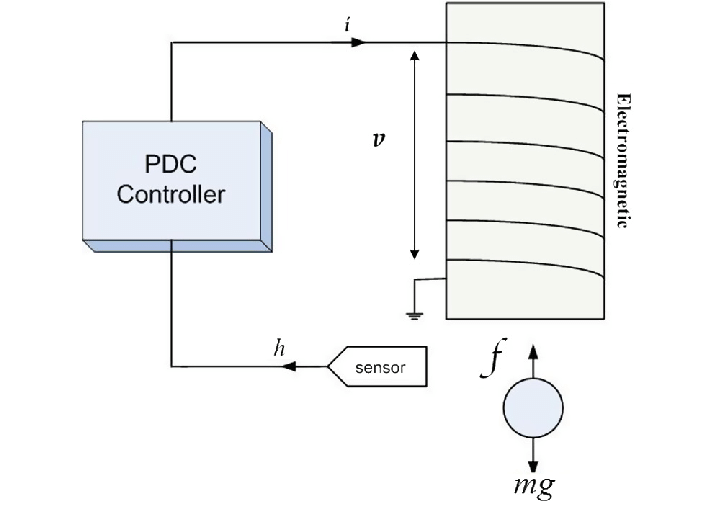
\includegraphics[width=0.5\linewidth]{./figs/Maglev-system-model}

Equação de movimento (lei de Newton):
\[
  m\ddot{x} = mg - f(x,I)
\]

Força magnética:
\[
  f(x,I) = \frac{kI^2}{(x+\mu)^2}
\]
Estados:

\begin{itemize}
\tightlist
\item
  Posição \(x\)
\item
  Velocidade \(v = \dot{x}\)
\end{itemize}

Equações de estado:

\begin{aligned}
  \dot{x} &= v\\
  \dot{v} &= g - f(x,I)/m = g - \frac{kI^2}{m(x+\mu)^2}
\end{aligned}

ou:
\[
  \begin{bmatrix} \dot{x} \\ \dot{v}\end{bmatrix} = \begin{bmatrix} v \\ g - \frac{kI^2}{m(x+\mu)^2}\end{bmatrix}
\]

A equação de saída é simplesmente
\[
 y = x
\]

Note que \(g\), \(k\), \(m\) e \(\mu\) são constantes.

\hypertarget{equiluxedbrio}{%
\section{Equilíbrio}\label{equiluxedbrio}}

A idéia de equilíbrio é fundamental em sistemas. Fisicamente, um estado de equilíbrio é aquele no qual o sistema não evoloui no tempo, permanece parado, seus sinais constantes, sem variação temporal.

Em sistemas não-lineares definimos matematicamente como ponto de equilíbrio os valores fixos do vetor de estados \(\mathbf{x}_0\) e de entrada \(\mathbf{u}_0\) que anulam a função \(\mathbf{F(x,u)}\), isto é, satisfazem:

\[
  \mathbf{F(x_0,u_0)} = \mathbf{0}
\]

O equilíbrio de um sistema possui interpretação física importante e está intimamente relacionado à estabilidade do sistema.

Um sistema não linear pode ter vários pontos de equilíbrio.

Um sistema LIT possui sempre um único ponto de equilíbrio dado por \(\mathbf{x_0=0}\) e \(\mathbf{u_0=0}\).

\textbf{Exemplo:} sistema MAGLEV

Em equilíbrio o sistema está totalmente parado, \(v=0\). O cilindro é mantido a uma distância \(x_0\) do imã, sob uma corrente \(I_0\).

As equações de equilíbrio são:

\begin{aligned}
  v &= 0\\
  f(x_0,I_0) &= mg
\end{aligned}

Apicando a equação da força magnética, temos a relação detalhada:
\[
  \frac{kI_0^2}{(x_0+\mu)^2} = mg \Rightarrow kI_0^2 = mg(x_0+\mu)^2
\]

\hypertarget{linearizauxe7uxe3o}{%
\section{Linearização}\label{linearizauxe7uxe3o}}

Um modelo linearizado é um modelo que tenta aproximar a evolução temporal de um sistema não-linear próximo do ponto de equilíbrio, isto é, supondo que os estados \(\mathbf{x}(t)\) não diferem muito de \(\mathbf{x_0}\).

Modelos linearizados também são chamados de modelo de perturbação ou modelo de pequenos sinais.

\[
  {\mathbf{x}} \approx \mathbf{x}_0+ \Delta \mathbf{x}
\]
com \(\Delta \mathbf{x}\) pequeno e \(\mathbf{x}_0\) o ponto de equilíbrio.

A maioria dos controladores que projetamos são lineares e o projeto deles é feito com base na aproximação linear do sistema.

Isso ocorre porque a teoria de sistemas lineares é bem consolidada: conseguimos resolver as equações analítica e numericamente. Para sistemas não lineares essa tarefa é muito mais complicada, quando não impossível.

Para linearizar um sistema, encontramos as aproximações em série de Taylor das funções \(\mathbf{F}\) e \(\mathbf{G}\), truncadas no termo linear, em torno do ponto de equilíbrio.

\begin{aligned}
  \mathbf{F(x,u)} &\approx \mathbf{F(x_0,u_0)} + \mathbf{A\,\Delta x} + \mathbf{B\,\Delta u}\\
  \mathbf{G(x,u)} &\approx \mathbf{G(x_0,u_0)} + \mathbf{C\,\Delta x} + \mathbf{D\,\Delta u}
\end{aligned}

onde as matrizes \(\mathbf{A}\), \(\mathbf{B}\), \(\mathbf{C}\) e \(\mathbf{D}\) são os seguintes Jacobianos.

\begin{aligned}
  \mathbf{A}  &= \left.\frac{\partial \mathbf{F}}{\partial \mathbf{x}}\right|_{\mathbf{x = x_0}, \mathbf{u=u_0}}\\
  \mathbf{B}  &= \left.\frac{\partial \mathbf{F}}{\partial \mathbf{u}}\right|_{\mathbf{x = x_0}, \mathbf{u=u_0}}\\
  \mathbf{C}  &= \left.\frac{\partial \mathbf{G}}{\partial \mathbf{x}}\right|_{\mathbf{x = x_0}, \mathbf{u=u_0}}\\
  \mathbf{D}  &= \left.\frac{\partial \mathbf{G}}{\partial \mathbf{u}}\right|_{\mathbf{x = x_0}, \mathbf{u=u_0}}
\end{aligned}

\textbf{Exemplo}: Sistema MAGLEV

\[
  \mathbf{F}(x,v,I) = \begin{bmatrix} v \\ g - \frac{kI^2}{m(x+\mu)^2}\end{bmatrix}
\]
Temos então:

\begin{aligned}
  f_1(x,v,I) &= v\\
  f_2(x,v,I) &= g - \frac{kI^2}{m(x+\mu)^2}
\end{aligned}

O ponto de equilíbrio é \((x_0,0,I_0)\) que satisfaz:
\[
kI_0^2 = mg(x_0+\mu)^2
\]

Os Jacobianos são:

\begin{aligned}
  \mathbf{A} &= \left.\frac{\partial \mathbf{F}}{\partial \mathbf{x}}\right|_{x=x_0, v=0, I=I_0} = \begin{bmatrix}\frac{\partial f_1}{\partial x} & \frac{\partial f_1}{\partial v} \\ \frac{\partial f_2}{\partial x} & \frac{\partial f_2}{\partial v}\end{bmatrix}\\
\mathbf{B} &= \left.\frac{\partial \mathbf{F}}{\partial \mathbf{u}}\right|_{x=x_0, v=0, I=I_0} = \begin{bmatrix} \frac{\partial f_1}{\partial I} \\ \frac{\partial f_2}{\partial I}\end{bmatrix}
\end{aligned}

\begin{aligned}
\frac{\partial f_1}{\partial x} &= 0\\
\frac{\partial f_1}{\partial v} &= 1\\
\frac{\partial f_2}{\partial x} &= \frac{2kI_0^2}{m(x_0+\mu)^3}=\lambda^2\\
\frac{\partial f_2}{\partial v} &= 0\\
\frac{\partial f_1}{\partial I} &= 0 \\
\frac{\partial f_2}{\partial I} &= \frac{2kI_0}{m(x_0+\mu)^2}=K_0
\end{aligned}

Assim, os sinais do MAGLEV podem ser aproximados pela seguinte dinâmica:

\begin{aligned}
  x &\approx x_0 + \Delta x\\
  v &\approx \Delta v
\end{aligned}

Onde os sinais auxiliares \(\Delta x\) e \(\Delta v\) são descritos pela equação de estados:

\begin{align}
\begin{bmatrix} \Delta\dot{x}\\ \Delta\dot{v}\end{bmatrix} = \begin{bmatrix}0 & 1 \\ \lambda^2 & 0\end{bmatrix}\begin{bmatrix}\Delta x\\ \Delta v\end{bmatrix} + \begin{bmatrix}0\\ K_0\end{bmatrix}\Delta I
\end{align}

\(\Delta I\) é a variação de corrente do imã em torno do valor de equilíbrio \(I_0\), \(\Delta I=I-I_0\).

\hypertarget{modelagem}{%
\chapter{Modelagem}\label{modelagem}}

Neste capítulo vamos estudar diferentes formas de obter equações de estados.

\hypertarget{sobre-a-nuxe3o-unicidade-da-representauxe7uxe3o-de-estados}{%
\section{Sobre a não unicidade da representação de estados}\label{sobre-a-nuxe3o-unicidade-da-representauxe7uxe3o-de-estados}}

Um sistema LIT pode possuir diferentes representações de estados. Isso depende de quais variáveis de estados são escolhidas para a representação. O mesmo sistema pode admitir diferentes conjuntos de estados.

Isso significa que um mesmo sistema pode possuir diferentes matrizes de representação, todas de mesma ordem. A representação não é única, por isso \emph{não unicidade}.

Isso não ocorre com a representação por função de transferência. Um sistema possui uma e apenas uma função de transferência padrão.

\hypertarget{equauxe7uxe3o-diferencial-simples}{%
\section{Equação diferencial simples}\label{equauxe7uxe3o-diferencial-simples}}

Para um sistema representado por uma EDO simples, sem derivadas do sinal de entrada, pode-se obter as equações de estado de um jeito bastante simples. Para isso basta escolher uma variável de estado como a derivada da outra, normalmente em sequência.

\textbf{Exemplo:}
\[
\dddot{y} + 6\ddot{y} + 11\dot{y} + 6y = 6u
\]
Sistema de 3a ordem, então definimos os estados como a saída e suas derivadas até ordem 2.

\begin{aligned}
    x_1 &=y\\
    x_2 &=\dot{y}\\
    x_3 &=\ddot{y}
\end{aligned}

Para um sistema de 2a ordem, definimos os estados como saída e sua derivada.

Generalizando, para um sistema de ordem \(n\), definimos a saída e todas as derivadas até ordem \(n-1\).

Para montar a equação de estados precisamos das derivadas de cada estado. Mas pela forma como definimos cada um, as duas primeiras derivadas podem ser obtidas em função da própria definição.

\begin{aligned}
    \dot{x}_1 &=\dot{y} = x_2\\
    \dot{x}_2 &=\ddot{y} = x_3
\end{aligned}

Por último, precisamos da derivada do último estado. Note que esta é:

\begin{aligned}
    x_3 &=\dddot{y}
\end{aligned}

que pode ser obtida da EDO original como:

\begin{aligned}
    \dddot{y} &= -6\ddot{y} - 11\dot{y} - 6y + 6u\\
    &= -6x_3 -11x_2 - 6x_1 + 6u
  \end{aligned}

Assim as equações de estado são:

\begin{aligned}
    \dot{x}_1 &=x_2\\
    \dot{x}_2 &= x_3\\
    \dot{x}_3 &=-6x_3 -11x_2 - 6x_1 + 6u
  \end{aligned}

Agora basta converter para o formato matricial. Na matriz \(\mathbf{A}\) o elemento da linha \(i\) e coluna \(j\) é o coeficiente da variável \(j\) na equação \(i\) (relativa a derivada da variável \(i\)). Na matriz \(\mathbf{B}\) o elemento da linha \(i\) é simplesmente o coeficiente de \(u\) na equação \(i\).

Para o exemplo, o resultado é:

\begin{aligned}
    \left[\begin{array}{c}\dot{x}_1\\
    \dot{x}_2\\
    \dot{x}_3\\ \end{array}\right] &= 
    \left[\begin{array}{rrr}1 & 0 & 0\\0 & 1 & 0 \\-6 & -11 & -6\end{array}\right]
    \left[\begin{array}{c}{x}_1\\ {x}_2\\ {x}_3\\ \end{array}\right] +
    \left[\begin{array}{c}0 \\ 0 \\ 6 \end{array}\right]u
\end{aligned}

Perceba que nossa escolha inicial da sequência de estados é arbitrária. Nada impede que façamos uma permutação. por exemplo:
\[
  \begin{aligned}
    x_3 &=y\\
    x_2 &=\dot{y}\\
    x_1 &=\ddot{y}
  \end{aligned}
\]
Tente verificar que neste caso, a equação de estados se tornaria:
\[
  \begin{aligned}
    \left[\begin{array}{c}\dot{x}_1\\
    \dot{x}_2\\
    \dot{x}_3\\ \end{array}\right] &= 
    \left[\begin{array}{rrr}-6 & -11 & -6\\ 1 & 0 & 0\\0 & 1 & 0\end{array}\right]
    \left[\begin{array}{c}{x}_1\\ {x}_2\\ {x}_3\\ \end{array}\right] +
    \left[\begin{array}{c}0 \\ 0 \\ 6 \end{array}\right]u
  \end{aligned}
\]

\hypertarget{diagramas-de-simulauxe7uxe3o}{%
\section{Diagramas de simulação}\label{diagramas-de-simulauxe7uxe3o}}

Em algumas ocasiões, modelos dinâmicos surgem ou são projetados a partir de um diagrama de simulação.

Esses são diagramas de blocos convencionais, tais como vistos em disciplinas anteriores, obedecendo às regras de simplificação normais.

Uma característica marcante é que eles são construídos apenas com 3 elementos: o integrador, o ganho e o somador.

Isso foi convecionado para, antigamente, facilitar a implementação com eletrônica analógica, i.e., amplificadores operacionais. Atualmente, utilizamos apenas para facilitar a escrita da equação de estados.

Os diagramas são uma forma inteligível de ler as relações entre os estados do sistema e assim deduzir as equações de estados.

\hypertarget{forma-canuxf4nica-de-controlador-fcc}{%
\section{Forma canônica de controlador (FCC)}\label{forma-canuxf4nica-de-controlador-fcc}}

A FCC é um tipo de representação útil principalmente para converter uma função de transferência em equação de estados.

Considere o seguinte exemplo:

\[
\begin{aligned}
G(s) &= \frac{s+2}{s^2+7s+12}
\end{aligned}
\]

Para construir um diagrama na forma canônica de controlador, faça o seguinte:

\begin{itemize}
\tightlist
\item
  Desenhe integradores em série, tantos quantos forem a ordem do sistema
\item
  A entrada será o sinal mais a esquerda. A saída, o mais a direita.
\item
  Realimente \textbf{todos} os integradores, cada um através de um ganho constante
\item
  As realimentações devem ser ligadas a um \textbf{único} somador posicionado na entrada do integrador mais a esquerda. Se quiser organizar melhor, divida o somador em outros de duas entradas, imediatamente abaixo
\item
  O valor de cada ganho de realimentação é o negativo de um coeficiente do denominador.
\item
  Utilize os coeficientes de \textbf{maior} potência de \(s\) para as ligações dos integradores mais perto da \textbf{entrada}
\item
  A saída do sistema é consturída a partir de um somador
\item
  Ao somador de saída, ligue as saídas de cada integrador através de um ganho constante
\item
  O valor de cada ganho é igual a um coeficiente do numerador
\item
  Utilize os coeficientes de \textbf{menor} potência de \(s\) para as ligações dos integradores mais perto da \textbf{saída}
\end{itemize}

\begin{figure}
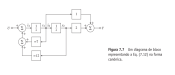
\includegraphics[width=1\linewidth]{./figs/Fig7.7} \caption{Diagrama de simulação}\label{fig:unnamed-chunk-8}
\end{figure}

Para o diagrama feito, as equações de estado são:

\[
\begin{aligned}
    \dot{x}_2&=x_{1}\\\dot{x}_1&=u - 7 x_{1} - 12 x_{2} 
\end{aligned}
\]

Logo a representação matricial é:

\[
\left[\begin{matrix}\dot{x}_1\\\dot{x}_2\end{matrix}\right]=\left[\begin{matrix}-7 & -12\\1 & 0\end{matrix}\right]\left[\begin{matrix}x_{1}\\x_{2}\end{matrix}\right]+\left[\begin{matrix}1\\0\end{matrix}\right]u
\]

Note que os estados foram ordenados da esquerda para a direita. \emph{O que aconteceria se tivéssemos nomeado ao contrário?}

\hypertarget{fcc-geral}{%
\section{FCC geral}\label{fcc-geral}}

Para um sistema geral de ordem \(n\), com função de transferência
\[
\begin{aligned}
    G(s) &= \frac{b_1s^{n-1}+b_2s^{n-2}+\ldots b_n}{s^n+a_1s^{n-1}+a_2s^{n-2}+\ldots + a_n}
\end{aligned}
\]

Perceba que o coeficiente de maior grau do denominador foi feito igual a \(1\).

As matrizes da forma canônica de controlador tem a seguinte estrutura

\[
\begin{aligned}
    \mathbf{A} &= \left[\begin{array}{cccccc} 
                  -a_1 & -a_2 & \ldots & a_{n-1} &-a_n\\
                     1 & 0 & \ldots & 0 & 0 \\
                     0 & 1 & \ldots & 0 & 0 \\
                     \vdots & \vdots & \ldots & \vdots& \vdots \\
                     0 & 0 & \ldots  & 1 & 0
    \end{array}\right]\\
    \mathbf{B} &= \left[\begin{array}{cccccc} 
                  1 \\ 0 \\ 0 \\ \vdots \\ 0 
    \end{array}\right]\\
    \mathbf{C} &= \left[\begin{array}{cccccc} 
                  b_1 & b_2 & \ldots & b_{n-1} & b_n 
    \end{array}\right]\\
    D &=0
\end{aligned}
\]

\textbf{Observações}

\begin{itemize}
\tightlist
\item
  Matriz \(\mathbf{A}\)

  \begin{itemize}
  \tightlist
  \item
    A primeira linha é dada pelos coeficientes do denominador, com sinal trocado, ordem decrescente de potência
  \item
    Abaixo da segunda linha temos uma matriz identididade e uma coluna de zeros
  \end{itemize}
\item
  Matriz \(\mathbf{B}\)

  \begin{itemize}
  \tightlist
  \item
    Primeiro elemento \(1\) e os demais zero
  \end{itemize}
\item
  Matriz \(\mathbf{C}\)

  \begin{itemize}
  \tightlist
  \item
    Coeficientes do numerador, sem troca de sinal, ordem decrescente de potência
  \end{itemize}
\item
  Termo \(D\)

  \begin{itemize}
  \tightlist
  \item
    Nulo (apenas se o grau do numerador for estritamente menor que o do denominador)
  \end{itemize}
\end{itemize}

\textbf{Observacão}: A função de transferência tem o grau do denominador estritamente maior que o do numerador. Caso não seja, é necessário fazer divisão longa antes de prosseguir. O termo quociente será a matriz \(D\).

\textbf{Exercício}: Ache as matrizes da forma de controlador do sistema:
\[
\begin{aligned}
    G(s) &= \frac{5s^2+8}{s(s+5)(s^2+9)}
\end{aligned}
\]

\hypertarget{forma-de-jordan-ou-modal}{%
\section{Forma de Jordan ou Modal}\label{forma-de-jordan-ou-modal}}

Na forma modal, os estados aparecem majoritariamente desacoplados, isto é, uma equação de estados depende apenas da sua própria variável de estado e do sinal de entrada.

Isso é possível sempre que o sistema tiver pólos reais e distintos.

Quando o sistema tiver pólos repetidos, haverá um pequeno acoplamento entre equações, mas apenas entre os estados referentes ao mesmo pólo.

Quando o sistema tiver pólos imaginários, as equações podem ser desacopladas, mas ao custo de ganhos imaginários.

Para eliminar os ganhos imaginários, podemos introduzir um pequeno acoplamento entre os estados associados aos pólos conjugados.

\textbf{Exemplo resolvido}:

\begin{figure}
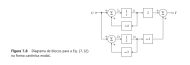
\includegraphics[width=1\linewidth]{./figs/Fig7.8} \caption{Diagrama em forma de Jordan}\label{fig:unnamed-chunk-9}
\end{figure}

Para o sistema da Fig 7.8.

\begin{aligned}
    \dot{z}_1 &= u - 4z_1\\
    \dot{z}_2 &= u - 3z_2\\
    y &= 2z_1-z_2
\end{aligned}

Uma consequência do desacoplamento é que matriz \(\mathbf{F}\) se torna \textbf{diagonal}.

\begin{aligned}
    \dot{\mathbf{x}} &= \left[\begin{array}{rr}-4 & 0\\0 & -3\end{array}\right]\mathbf{x}+\left[\begin{array}{r}1\\1\end{array}\right]u\\
    y &= \left[\begin{array}{rr}2 & -1\end{array}\right]\mathbf{x}
\end{aligned}

A forma modal é útil para determinar rápida e intuitivamente uma propriedade chamada controlabilidade. O sistema é não-controlável quando o sinal de controle não consegue ``chegar'' até um determinado integrador por nenhum caminho.

Algumas observações importantes:

\begin{enumerate}
\def\labelenumi{\arabic{enumi}.}
\tightlist
\item
  Um sistema pode perder controlabilidade quando na sua função de transferência há algum cancelamento entre pólos e zeros.
\item
  Para achar a forma modal a partir da função de transferência, use expansão em frações parciais
\end{enumerate}

\hypertarget{puxf3los-reais-e-distintos}{%
\section{Pólos reais e distintos}\label{puxf3los-reais-e-distintos}}

\begin{itemize}
\tightlist
\item
  Ache a expansão em frações parciais da função de transferência
\item
  Faça um diagrama para cada uma das parcelas da expansão
\item
  Nomeie os estados (saída dos integradores) e monte as equações normalmente
\end{itemize}

\textbf{Mais um exemplo de modal}

\begin{aligned}
    G(s) &=\frac{s+3}{(s+1)(s+5)(s-9)}
\end{aligned}

Precisamos primeiro expandir e achar os resíduos (frações parciais). É possível fazer isso usando a função ``residue'' do módulo \emph{scipy.signal}. A funçao ``apart'' do módulo \emph{sympy} também resolve o problema, embora nem sempre da forma esperada em problemas de engenharia.

\begin{Shaded}
\begin{Highlighting}[]
\ImportTok{import}\NormalTok{ scipy.signal }\ImportTok{as}\NormalTok{ sig}
\ImportTok{import}\NormalTok{ numpy }\ImportTok{as}\NormalTok{ np}
\NormalTok{num }\OperatorTok{=}\NormalTok{ [}\DecValTok{1}\NormalTok{,}\DecValTok{3}\NormalTok{]}
\NormalTok{den }\OperatorTok{=}\NormalTok{ np.poly([}\OperatorTok{{-}}\DecValTok{1}\NormalTok{,}\OperatorTok{{-}}\DecValTok{5}\NormalTok{,}\DecValTok{9}\NormalTok{])}
\NormalTok{r,p,k }\OperatorTok{=}\NormalTok{ sig.residue(num,den)}
\NormalTok{r }\OperatorTok{=}\NormalTok{ r.}\BuiltInTok{round}\NormalTok{(decimals}\OperatorTok{=}\DecValTok{4}\NormalTok{)}
\NormalTok{p }\OperatorTok{=}\NormalTok{ p.}\BuiltInTok{round}\NormalTok{(decimals}\OperatorTok{=}\DecValTok{4}\NormalTok{)}
\BuiltInTok{print}\NormalTok{(r)}
\end{Highlighting}
\end{Shaded}

\begin{verbatim}
## [-0.05   -0.0357  0.0857]
\end{verbatim}

\begin{Shaded}
\begin{Highlighting}[]
\BuiltInTok{print}\NormalTok{(p)}
\end{Highlighting}
\end{Shaded}

\begin{verbatim}
## [-1. -5.  9.]
\end{verbatim}

Logo:
\[
    G(s) = \frac{-0.05}{s+1}-\frac{0.03}{s+5}+\frac{0.08}{s-9}
\]

O diagrama para a representação de cada modo está a seguir

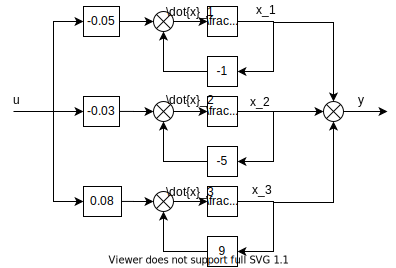
\includegraphics[width=1\linewidth]{./figs/modal1}

As equações de estado vão ser (\textbf{verifique você mesmo!}):
\[
    \dot{x}_1 = -x_1-0.05u
\]

\[
    \dot{x}_2 = -5x_2-0.03u
\]

\[
    \dot{x}_3 = 9x_3+0.08u
\]

A equação de saída é:
\[
    y = x_1+x_2+x_3
\]

Por fim, a representação matricial:
\[
    \dot{\mathbf{x}} = \left[\begin{array}{rrr}
    -1 & 0 & 0\\
    0 & -5 & 0\\
    0 & 0 & 9
    \end{array}
    \right]\mathbf{x} +
    \left[\begin{array}{r}
    1 \\
    1 \\
    1 
    \end{array}\right]u
\]

E a equação de saída.

\begin{aligned}
    y = \left[\begin{array}{ccc}-0.05 & -0.03 & 0.08\end{array}\right]\mathbf{x}
\end{aligned}

\hypertarget{forma-de-jordan-com-polos-reais-e-repetidos}{%
\section{Forma de Jordan com polos reais e repetidos}\label{forma-de-jordan-com-polos-reais-e-repetidos}}

Suponha que:

\begin{aligned}
    G(s) &= \frac{16s}{(s+3)^2(s+5)}
\end{aligned}

Vamos calcular rapidamente os resíduos e a expansão:

\begin{Shaded}
\begin{Highlighting}[]
\NormalTok{num }\OperatorTok{=}\NormalTok{ np.array([}\DecValTok{16}\NormalTok{,}\DecValTok{0}\NormalTok{])}
\NormalTok{den }\OperatorTok{=}\NormalTok{ np.convolve([}\DecValTok{1}\NormalTok{,}\DecValTok{3}\NormalTok{],[}\DecValTok{1}\NormalTok{,}\DecValTok{3}\NormalTok{])}
\NormalTok{den }\OperatorTok{=}\NormalTok{ np.convolve(den,[}\DecValTok{1}\NormalTok{,}\DecValTok{5}\NormalTok{])}
\NormalTok{r,p,k }\OperatorTok{=}\NormalTok{ sig.residue(num,den)}
\BuiltInTok{print}\NormalTok{(r)}
\end{Highlighting}
\end{Shaded}

\begin{verbatim}
## [ 20. -24. -20.]
\end{verbatim}

\begin{Shaded}
\begin{Highlighting}[]
\BuiltInTok{print}\NormalTok{(p)}
\end{Highlighting}
\end{Shaded}

\begin{verbatim}
## [-3. -3. -5.]
\end{verbatim}

Então:
\[
\begin{aligned}
    G(s) &= \frac{20}{(s+3)}-\frac{24}{(s+3)^2}-\frac{20}{s+5}
\end{aligned}
\]

Observe no diagrama como devemos implementar o termo quadrático:

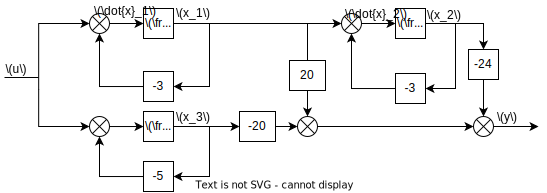
\includegraphics[width=1\linewidth]{./figs/modal3}

Observe que os estágios correspondentes ao polo repetido ficam em série, e não em paralelo, diferente dos outros.

\textbf{Exercício: escreva a representação matricial}

\hypertarget{transformauxe7uxe3o-de-estado}{%
\section{Transformação de estado}\label{transformauxe7uxe3o-de-estado}}

Uma única função de transferência pode ter diferentes representações de estado (matrizes)

Quando mudamos de uma representação para outra, as matrizes mudam, e os estados \textbf{não são mais os mesmos}. Eles adquirem outro significado físico. No entanto, as características intrínsecas do sistema, tais como pólos, zeros, estabilidade e outras permanecem as mesmas.

A explicação matemática para isso é a teoria de transformações lineares.

Supondo que a representação ``velha'' seja:

\begin{aligned}
    \mathbf{\dot{x}} &= \mathbf{Ax+B}u\\
    y &= \mathbf{Cx}+Ju
\end{aligned}

A mudança para um novo vetor de estados, digamos \(\mathbf{z}\), é representada por uma transformação linear:

\begin{aligned}
    \mathbf{x} &= \mathbf{Tz}
\end{aligned}

onde \(\mathbf{T}\) é uma matriz quadrada de ordem \(n\), inversível (ou seja, é possível ``ir'' e ``voltar'' com a mudança).

Esperamos que, usando o novo vetor de estados \(\mathbf{z}\), a representação seja algo como:

\begin{aligned}
    \mathbf{\dot{z}} &= \mathbf{A_nz+B_n}u\\
    y &= \mathbf{C_nz}+D_nu
\end{aligned}

Pode-se mostrar que a representação ``nova'' se relaciona com a ``velha'', usando a matriz de transformação \(\mathbf{T}\) da seguinte forma:

\begin{aligned}
    \mathbf{A}_n &= \mathbf{T^{-1}AT}\\
    \mathbf{B}_n &= \mathbf{T^{-1}B}\\
    \mathbf{C}_n &= \mathbf{CT}\\
    D_n &= D
\end{aligned}

A transformação para forma de Jordan, em particular, é um procedimento que chamamos de diagonalização

\hypertarget{dica-uxfatil-matriz-inversa-de-segunda-ordem}{%
\section{Dica útil: Matriz inversa de segunda ordem}\label{dica-uxfatil-matriz-inversa-de-segunda-ordem}}

Para fazer transformações em sistemas de ordem 2, precisamos da inversa da matriz de transformação.

Um regra rápida para achar a inversa de 2a ordem é:

\begin{enumerate}
\def\labelenumi{\arabic{enumi}.}
\tightlist
\item
  Troque a ordem dos elementos da diagonal principal
\item
  Inverta o sinal dos elementos não diagonais
\item
  Divida a matriz inteira pelo determinante da matriz original (supondo que ele não é zero)
\end{enumerate}

\begin{aligned}
    \left[\begin{array}{cc} a&b\\c&d \end{array}\right]^{-1} &= \frac{\left[\begin{array}{cc} d&-b\\-c&a \end{array}\right]}{ad-bc}
\end{aligned}

\textbf{Lembre-se que isso só vale para matriz de ordem 2!}

\textbf{Exercício}: para a função de transferência

\begin{aligned}
    G(s) =\frac{3s^2-1}{(s+1)(s+7)(s+5)}
\end{aligned}

\begin{enumerate}
\def\labelenumi{\arabic{enumi}.}
\tightlist
\item
  Faça o diagrama de blocos da forma de controlador
\item
  Obtenha as matrizes da forma de controlador
\item
  Obtenha as matrizes da forma modal
\item
  Ache as matrizes se aplicada a transformação
\end{enumerate}

\begin{aligned}
    \mathbf{T} =\left[\begin{array}{cc}1&-1\\1&1 \end{array}\right]
\end{aligned}

\hypertarget{puxf3los-complexos-conjugados}{%
\section{Pólos complexos conjugados}\label{puxf3los-complexos-conjugados}}

Quando os polos são complexos, somos tentados a usar ganhos complexos no diagrama de blocos, o que não é possível de realizar fisicamente.

Quando há polos complexos e, consequentemente, resíduos complexos, podemos fazer um artifício baseado na própria expansão em frações para nos ``livrarmos'' de qualquer número complexo presente.

Suponha, por exemplo:

\begin{aligned}
    G(s) &= \frac{100}{s(s^2+2s+5)}
\end{aligned}

A expansão em frações parciais dessa função é:

\begin{aligned}
    G(s) &= \frac{20}{s}+\frac{-10+j5}{s+1-j2}+\frac{-10-j5}{s+1+j2}
\end{aligned}

Os pólos complexos usam ganhos de realimentação e de saída complexos. Para evitar isso, podemos usar um artifício que acopla os modos complexos entre si, mas continuando isolados dos outros modos do sistema

Para um caso geral de conjugados

\begin{aligned}
    \frac{a+jb}{s-\sigma-j\omega}+\frac{a-jb}{s-\sigma+j\omega}
\end{aligned}

O diagrama de blocos (dedução um pouco trabalhosa) equivalente é:

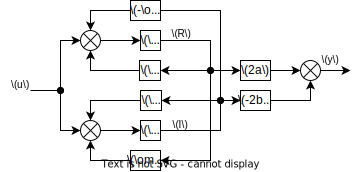
\includegraphics[width=1\linewidth]{./figs/JordanComplexos}

As equações de estado são as seguintes:

\begin{aligned}
    \dot{R} &= \sigma R-\omega I + u\\
    \dot{I} &= \omega R-\sigma I + u\\
    y &= 2a\, R -2b\, I
\end{aligned}

Assim, a contribuição do par conjugado para a forma modal é a seguinte:

\begin{itemize}
\tightlist
\item
  Na matriz de estados, encaixe a seguinte matrix \(2\times 2\) feita a partir das partes real e imaginária dos pólos complexos

  \begin{aligned}
    \left[\begin{array}{cc} \sigma & -\omega\\ \omega & \sigma\end{array}\right]
  \end{aligned}
\item
  Na matriz de entrada, a contribuição é apenas um vetor coluna de 1's
\item
  Na matriz de saída, a contribuição é uma linha de dois elementos construído a partir das partes real e imaginária do resíduo complexo

  \begin{aligned}
    \left[\begin{array}{cc} 2a & -2b\end{array}\right]
  \end{aligned}
\end{itemize}

Voltando ao exemplo\ldots{}

\begin{aligned}
    G(s) &= \frac{20}{s}+\frac{-10+j5}{s+1-j2}+\frac{-10-j5}{s+1+j2}
\end{aligned}

Para a parcela complexa, vamos tomar como referência o pólo \(s=-1+j2\). Para este, \(\sigma = -1\) e \(\omega=2\)

O resíduo complexo correspondente é \(-10+j5\). Então, neste caso: \(a=-10\) e \(b=5\)

Assim as equações de estado serão:

\begin{aligned}
    \dot{x}_1 &= u\\
    \dot{x}_2 &= -x_2-2x_3+u\\
     \dot{x}_3 &= 2x_2-x_3+u\\
     y &= 20x_1 -20x_2+10x_3
\end{aligned}

\textbf{Construa as matrizes a partir daqui. Observe que a matriz de estados não é mais diagonal (mas é quase)}

\hypertarget{anuxe1lise-de-sistemas-com-espauxe7o-de-estados}{%
\chapter{Análise de sistemas com espaço de estados}\label{anuxe1lise-de-sistemas-com-espauxe7o-de-estados}}

Dada uma entrada \(u(t)\) e uma condição inicial dos estados \(\mathbf{x}(0)\), podemos resolver a equação diferencial (matricial) dos estados e determinar a saída do sistema.

Isso pode ser feito com a transformada de Laplace da mesma forma como se fosse uma equação escalar. Devemos apenas atentar que para uma equação matricial, a divisão é substituída pela multiplicação por matriz inversa.

\begin{aligned}
    \mathbf{\dot{x}} &= \mathbf{Ax+B}u\\
    \mathcal{L}\{\mathbf{\dot{x}}\} &= \mathcal{L}\{\mathbf{Ax+B}u\}\\
    s\mathbf{X}(s)-\mathbf{x}(0) &= \mathbf{AX}(s)+\mathbf{B}U(s)\\
    s\mathbf{X}(s)-\mathbf{AX}(s)&=\mathbf{x}(0)+\mathbf{B}U(s)\\
    (s\mathbf{I-A})\mathbf{X(s)} &= \mathbf{x}(0)+\mathbf{B}U(s)\\
    \mathbf{X(s)} &= (s\mathbf{I-A})^{-1}\mathbf{x}(0)+(s\mathbf{I-A})^{-1}\mathbf{B}U(s)\\
\end{aligned}

O termo \((s\mathbf{I-A})^{-1}\mathbf{x}(0)\) é a resposta de entrada nula, devido sua independência da função de entrada.

O termo \((s\mathbf{I-A})^{-1}\mathbf{B}U(s)\) é a resposta de estado nulo, devido sua independência das condições iniciais.

Para determinar os estados no domínio do tempo \(\mathbf{x}(t)\) bastaria tirar a transformada inversa. Assim teríamos a resposta de cada um dos estados em função do tempo.

\hypertarget{sinal-de-sauxedda-e-funuxe7uxe3o-de-transferuxeancia}{%
\section{Sinal de saída e função de transferência}\label{sinal-de-sauxedda-e-funuxe7uxe3o-de-transferuxeancia}}

Olhando agora o sinal de saída:

\begin{aligned}
    y &= \mathbf{Cx} + Du\\
    Y(s) &= \mathbf{CX(s)} + DU(s)
\end{aligned}

Substituindo o que encontramos para \(\mathbf{X}(s)\):

\begin{aligned}
    Y(s) &= \mathbf{C}(s\mathbf{I-A})^{-1}\mathbf{x}(0)+\mathbf{C}(s\mathbf{I-A})^{-1}\mathbf{B}U(s) + DU(s)
\end{aligned}

Colocando \(U(s)\) em evidência agora:

\begin{aligned}
    Y(s) &= \mathbf{C}(s\mathbf{I-A})^{-1}\mathbf{x}(0)+\left[\mathbf{C}(s\mathbf{I-A})^{-1}\mathbf{B} + D\right]U(s)
\end{aligned}

Quando as condições iniciais são nulas \(\mathbf{x}(0)=\mathbf{0}\), o termo que sobra é um escalar:

\begin{aligned}
    Y(s) &= \left[\mathbf{C}(s\mathbf{I-A})^{-1}\mathbf{B} + D\right]U(s)\\
    \frac{Y(s)}{U(s)} &= \mathbf{C}(s\mathbf{I-A})^{-1}\mathbf{B} + D
\end{aligned}

Reconhecemos a última equação como a função de transferência do sistema definida em termos das matrizes da representação de espaço de estados.

\hypertarget{puxf3los-de-um-sistema-no-espauxe7o-de-estados-autovalores}{%
\section{Pólos de um sistema no espaço de estados (Autovalores)}\label{puxf3los-de-um-sistema-no-espauxe7o-de-estados-autovalores}}

Na equação da função de transferência, o termo principal é \((s\mathbf{I-A})^{-1}\). Sabemos que a inversa de qualquer matriz pode ser descrita como sua adjunta divido pelo seu determinante. O que vai sobrar no denominador da função de transferência, portanto, é \(\det (s\mathbf{I-A})\).

Sabemos que os pólos são as raízes do denominador de uma função de transferência. Ora, se o denominador é dado pelo determinante acima, então os pólos do sistema são dados pelas soluções da equação:

\begin{aligned}
\det (s\mathbf{I-A}) = 0
\end{aligned}

Os valores de \(s\) que satisfazem essa equação são chamados em álgebra linear de \textbf{autovalores da matriz} e de desempenham um papel importante em vários problemas de Engenharia.

Em Python vc pode calcular os autovalores do sistema usando a funçao ``pole()'' da biblioteca \emph{control}, ou usar a biblioteca \emph{linalg} do NumPy para resolver o problema de autovalor diretamente na matriz de estados do sistema. Note, porém, que a função ``eig()'' do NumPy devolve não apenas os autovalores, mas também os \href{https://pt.wikipedia.org/wiki/Autovalores_e_autovetores}{autovetores} associados também.

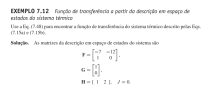
\includegraphics[width=1\linewidth]{./figs/Ex7.12}

Solução manual (você precisa saber fazer manualmente \emph{pelo menos} os casos de ordem 2):

\begin{aligned}
    s\mathbf{I-A} &= s\left[\begin{array}{cc}1 & 0\\0 & 1\end{array}\right]-\left[\begin{array}{cc}-7 & -12\\1 & 0\end{array}\right]\\
    &= \left[\begin{array}{cc}s+7 & 12\\-1 & s\end{array}\right]
\end{aligned}

A inversa da matriz é:

\begin{aligned}
    (s\mathbf{I-A})^{-1} &= \frac{\left[\begin{array}{cc}s & -12\\1 & s+7\end{array}\right]}{s(s+7)+12}
\end{aligned}

Faz-se agora o produto pela esquerda:

\begin{aligned}
    \mathbf{C}(s\mathbf{I-A})^{-1} &= \frac{\left[\begin{array}{cc}1 & 2\end{array}\right]\left[\begin{array}{cc}s & -12\\1 & s+7\end{array}\right]}{s(s+7)+12}\\
    &= \frac{\left[\begin{array}{cc}s+2 & 2s+2\end{array}\right]}{s^2+7s+12}
\end{aligned}

E o resultado com o produto pela direita:

\begin{aligned}
    \mathbf{C}(s\mathbf{I-A})^{-1}\mathbf{B} &= \frac{\left[\begin{array}{cc}s+2 & 2s+2\end{array}\right]\left[\begin{array}{c}1 \\ 0\end{array}\right]}{s^2+7s+12}\\
    & = \frac{s+2}{s^2+7s+12}
\end{aligned}

\textbf{Exercício}: Calcule manualmente e confira sua resposta com Python, a função de transferência do sistema

\begin{aligned}
\dot{\mathbf{x}} &= \left[\begin{array}{cc}-1 & 7\\ 9 & 0\end{array}\right]\mathbf{x} + \left[\begin{array}{cc} 5 \\ -3\end{array}\right]u\\
y &= \left[\begin{array}{cc}3 & 2\end{array}\right]\mathbf{x} 
\end{aligned}

\hypertarget{zeros-do-sistema}{%
\section{Zeros do sistema}\label{zeros-do-sistema}}

Na descrição entrada-saída (função de transferência) de um sistema, definimos zeros de uma forma bem matemática: são as raízes do numerador.

No entanto, os zeros possuem uma definição um pouco mais física. São chamados zeros os modos (exponenciais) que, se colocados na entrada do sistema, produzem uma saída identicamente nula. Isso permite estabelecer as expressões que definem os zeros do sistema em função das matrizes de espaço de estados.

Para achar os zeros, basta resolver a equação polinomial:

\begin{aligned}
\det\,\left[\begin{array}{cc}s\mathbf{I-A} & -\mathbf{B}\\ \mathbf{C} & D\end{array}\right]=0 
\end{aligned}

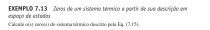
\includegraphics[width=1\linewidth]{./figs/Ex7.13}

\textbf{Solução}: Precisamos montar a matriz. No caso, já calculamos \(s\mathbf{I-A}\) no exemplo anterior, então basta concatenar as demais:

\begin{aligned}
    s\mathbf{I-A} &= \left[\begin{array}{cc}s+7 & 12\\-1 & s\end{array}\right]\\
    \Rightarrow \left[\begin{array}{ccc}s\mathbf{I-A} & -\mathbf{B}\\ \mathbf{C} & D\end{array}\right]&=
    \left[\begin{array}{ccc}s+7 & 12 & -1\\-1 & s & 0\\ 1 & 2 & 0 \end{array}\right]
\end{aligned}

Basta agora calcular o determinante.

\begin{aligned}
    \det \left[\begin{array}{ccc}s+7 & 12 & 1\\-1 & s & 0\\ 1 & 2 & 0 \end{array}\right] &= 
    \det \left[\begin{array}{cc}-1 & s \\ 1 & 2 \end{array}\right] = -2-s 
\end{aligned}

Igualando a zero, temos:

\begin{aligned}
    -2-s =0 \Rightarrow s = -2
\end{aligned}

Em Python, a função ``zero()'' é capaz de determinar os zeros a partir da representação do sistema

\hypertarget{estabilidade-no-espauxe7o-de-estados}{%
\section{Estabilidade no espaço de estados}\label{estabilidade-no-espauxe7o-de-estados}}

O conceito de estabilidade no espaço de estados é um pouco diferente do que aprendemos na representação entrada-saída.

A estabilidade é relativa a um ponto de equilíbrio do sistema.

Um sistema é estável se, dada uma condição inicial \(\mathbf{x}(0)\) próxima do ponto de equilíbrio, o estado \(\mathbf{x}(t)\) do sistema retorna para o ponto de equilíbrio inicial e ali permanece.

Um sistema linear possui apenas um ponto de equilíbrio, o vetor nulo \(\mathbf{x}= \left[\begin{array}{cccc}0 & 0 & \ldots & 0\end{array}\right]\).

É fácil de verificar que esse é um ponto de equilíbrio. Dada a equação de estados

\begin{aligned}
    \mathbf{\dot{x}} &= \mathbf{Ax+B}u
\end{aligned}

vemos que se \(u=0\) e se \(\mathbf{x=0}\), então todo o lado direito se anula, o que implica que \(\mathbf{\dot{x}=0}\). Ou seja, o sistema não evolui com o tempo, fica sempre no ``mesmo lugar''.

Um sistema linear será estável se, dada uma condição inicial diferente de zero do vetor de estados, o vetor \(\mathbf{x}(t)\) voltar para zero em um determinado intervalo de tempo.

Como já sabemos, o sistema é estável quando todos os seus pólos estão no semi-plano esquerdo (SPE). Como no espaço de estados os pólos são autovalores da matriz de estados \(\mathbf{A}\), então o sistema será estável se todos esses autovalores tiverem parte real estritamente negativa.

Isso garante que quando passar um longo tempo, isto é, \(t\rightarrow \infty\), os estados tenderão a zero, ou seja \(\mathbf{x}(t) \rightarrow \mathbf{0}\). Isso é chamado também de \textbf{estabilidade assintótica}.

\textbf{Exemplo:} verifique se o sistema abaixo é estável

\begin{aligned}
    \dot{\mathbf{x}}= \left[\begin{array}{cc}0 &1\\ -3 & -7\end{array}\right]\mathbf{x} +
    \left[\begin{array}{c}1\\ 2\end{array}\right]u
\end{aligned}

Solução manual:
\begin{align}
  s\mathbf{I-A} &=  s \left[\begin{matrix}1 & 0\\0 & 1\end{matrix}\right] -  \left[\begin{matrix}0 & 1\\-3 & -7\end{matrix}\right] \\
  &=  \left[\begin{matrix}s & 0\\0 & s\end{matrix}\right] - \left[\begin{matrix}0 & 1\\-3 & -7\end{matrix}\right] \\
  &=  \left[\begin{matrix}s & -1\\3 & s + 7\end{matrix}\right] 
\end{align}

Logo:
\begin{align}
  |s\mathbf{I-A}| &= \left| \left[\begin{matrix}s & -1\\3 & s + 7\end{matrix}\right] \right|\\
  &= s^{2} + 7 s + 3
\end{align}

Igualando o polinômio característico a zero temos as raízes \(s = -6.541\) e \(s = -0.4586\). Ambas possuem parte real negativa, logo o sistema é estável.

Usando Python:

\begin{Shaded}
\begin{Highlighting}[]
\ImportTok{import}\NormalTok{ numpy }\ImportTok{as}\NormalTok{ np}

\NormalTok{A }\OperatorTok{=}\NormalTok{ np.array([[}\DecValTok{0}\NormalTok{,}\DecValTok{1}\NormalTok{],[}\OperatorTok{{-}}\DecValTok{3}\NormalTok{, }\OperatorTok{{-}}\DecValTok{7}\NormalTok{]])}
\NormalTok{np.linalg.eig(A)[}\DecValTok{0}\NormalTok{]}
\end{Highlighting}
\end{Shaded}

\begin{verbatim}
## array([-0.45861873, -6.54138127])
\end{verbatim}

A função ``eig'' do submódulo ``numpy.linalg'' calcula os autovalores e autovetores de uma matriz quadrada. O primeiro argumento de saída (por isso o ``{[}0{]}'') fornece os autovalores, que neste caso correspondem ao que foi calculado manualmente.

\hypertarget{realimentauxe7uxe3o-de-estados}{%
\chapter{Realimentação de estados}\label{realimentauxe7uxe3o-de-estados}}

A principal técnica de controle em espaço de estados é o que chamamos de
``realimentação de estados''.

A estratégia básica é fazer a lei de controle \(u\) ser proporcional ao
vetor de estados.
\begin{align*}
    u = -\mathbf{Kx}
\end{align*}

Isto lembra um pouco o controle proporcional: realimentação negativa
e o controlador é apenas uma constante. Mas a diferença básica é que,
como o \(\mathbf{x}\) é um vetor, o controlador \(\mathbf{K}\) tem que ser
um vetor também.

O sinal de controle é um escalar. Sendo \(\mathbf{x}\) um vetor coluna de
\(n\) elementos, então \(\mathbf{K}\) deve ser um vetor linha de \(n\)
elementos. Assim:
\begin{align*}
    \mathbf{K}= \left[\begin{array}{cccc}K_1 & K_2 & \ldots & K_n\end{array}\right]
\end{align*}

O objetivo inicial da realimentação de estados é fazer com que os
estados do sistema caminhem para zero (ponto de equilíbrio) a partir de
um estado inicial \(\mathbf{x}(0)\neq \mathbf{0}\), em regime permanente
(isto é, passado um longo tempo). Esse problema é chamado de
\textbf{regulação}.

É possível mostra que se o controlador é capaz de fazer regulação de
estados, podemos fazer a saída atingir qualquer valor, que é o objetivo
do sistema de controle.

\textbf{Observação importante}: para o algoritmo funcionar supomos que
\textbf{todos} os estados são conhecidos para calcular a ação de controle.

Isso quase sempre não é verdade. Os estados são grandezas internas que,
às vezes, nem conseguimos medir. Mas mesmo quando é possível, pode não
ser economicamente viável comprar sensores para medir todos os estados (um sistema de ordem elevada). O único sinal que está disponível, por definição, é o sinal de saída.

Na prática o que se faz é construir um sistema auxiliar que
forneça uma \emph{estimativa} dos estados reais a partir do sinal de saída.
Esse sistema é conhecido como estimador ou observador de estados. O projeto e análise do observador de estados será visto mais a frente.

\textbf{Por enquanto vamos considerar que é possível medir todos os estados do
sistema para fazer a realimentação}

\hypertarget{anuxe1lise-da-realimentauxe7uxe3o-de-estados}{%
\section{Análise da realimentação de estados}\label{anuxe1lise-da-realimentauxe7uxe3o-de-estados}}

Para entender como projetar o controlador, precisamos entender o que acontece com o sistema quando a estratégia é implementada.

Seja um sistema:
\begin{align*}
    \mathbf{\dot{x}} &= \mathbf{Ax+B}u
\end{align*}

Se usarmos a lei de controle \(u = -\mathbf{Kx}\), a equação deixará de
ter entrada, podendo ser resolvida a partir da condição inicial.

\begin{align*}
    \mathbf{\dot{x}} &= \mathbf{Ax+B(-Kx)}\\
    &= \mathbf{Ax-BKx}\\
    &= \mathbf{(A-BK)x}\\
    \mathbf{\dot{x}} &= \mathbf{A}_m \mathbf{x}
\end{align*}

Vamos chamar matriz \(\mathbf{A}_m\) de ``matriz de malha fechada''.

A última equação é uma EDO que não possui entrada, então só tem sentido
resolvê-la para uma condição inicial \(\mathbf{x}(0)\) diferente de zero.

A condição necessária para que os estados do sistema caminhem para zero
em regime permanente é apenas que o sistema em malha fechada seja
estável, isto é, \textbf{todos} os autovalores da matriz \(\mathbf{A}_m\) devem
ter parte real estritamente negativa.

Além de estabilidade, é também desejado que a convergência dos estados
para zero seja feita com critérios de velocidade e oscilação específicos
do projeto. Isso é equivalente a satisfazer as condições de overshoot,
tempo de acomodação e dominância.

As condições de projeto são definidas em termos de pólos de malha fechada bem selecionados. Esses pólos determinam um polinômio de malha fechada \(\alpha (s)\).

Sendo assim, o problema de regulação é enunciado como: \emph{achar a matriz}
\(\mathbf{K}\), tal que estejam no semi-plano esquerdo todas as raizes da
equação:
\begin{align}
    \det (s\mathbf{I-A_m})= \det (s\mathbf{I-A+BK})=\alpha (s)
\end{align}

\textbf{Exemplo}

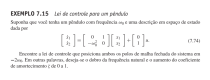
\includegraphics[width=1\linewidth]{./figs/Ex7.15}

Problema de segunda ordem, então: \(\mathbf{K} = \begin{bmatrix} k_1 & k_2\end{bmatrix}\).

Matriz de malha fechada:
\begin{align}
  \mathbf{A-BK} = \left[\begin{matrix}0 & 1\\- \omega_{0}^{2} - k_{1} & - k_{2}\end{matrix}\right]
\end{align}

Polinômio característico de malha fechada:
\[
  |s\mathbf{I-A+BK}| = \omega_{0}^{2} + k_{1} + k_{2} s + s^{2}
\]

Polinômio mônico desejado, com dois polos em \(-2\omega_0\):
\[
  \alpha(s) = 4 \omega_{0}^{2} + 4 \omega_{0} s + s^{2}
\]

Igualando termo a termo:
\begin{align}
  k_1 + \omega_0^2 &= 4\omega_0^2 \Rightarrow k_1 = 3\omega_0^2\\
  k_2 &= 4\omega_0
\end{align}

O livro mostra uma simulação da resposta desse sistema para
\(\omega_0=1\).

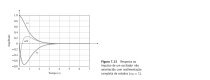
\includegraphics[width=1.2\linewidth]{./figs/Fig7.13}

Repare que os gráficos mostram, em função do tempo, os
dois estados. Note que nenhum dos sinais oscila. Isso porque as características dos pólos que foram alocados são válidas para todos os estados e a saída do
sistema.

\textbf{Exercício}

Ache a forma de controlador do sistema
\begin{align}
    G(s) = \frac{20}{(s+1)(s+2)}
\end{align}

Depois, projete um controlador de realimentação de estados que posicione
os pólos em \(-3\pm j5\)

\hypertarget{forma-canuxf4nica-de-controlador}{%
\section{Forma canônica de controlador}\label{forma-canuxf4nica-de-controlador}}

O exemplo anterior ilustra bem a solução do problema de realimentação de
estados. Porém, ele é simples demais:

\begin{itemize}
\tightlist
\item
  Ele é de ordem baixa (2). Na
  prática, os sistemas podem ser de ordem bem mais elevada
  -Em um problema de ordem mais alta, o trabalho seria muito maior e a solução
  desenvolvida, inviável
\item
  Além disso, em um problema real temos também
  que nos preocupar com questões numéricas de arredondamento.
\end{itemize}

A primeira forma de lidar com problemas de ordem mais alta é transformar
o sistema para forma canônica de controlador.

Usar essa forma é vantajoso porque ela simplifica as equações dos ganhos
na hora que igualamos os polinômios desejado e de projeto. Isso permite
encontrar os ganhos com equações mais simples, geralmente fazendo
substituições sucessivas.

Normalmente, a forma mais fácil de mudar para a forma de controlador é
achando a função de transferência do sistema e usando as regras práticas
de inspeção do numerador e denominador.

Isso pode ser um pouco trabalhoso para sistemas de ordem elevada.

\hypertarget{muxe9todo-de-ackermann}{%
\section{Método de Ackermann}\label{muxe9todo-de-ackermann}}

Uma maneira mais direta e geral de projetar a realimentação de estados é
usar o método de Ackerman. Ele consiste de aplicar a expressão:
\begin{align}
    \mathbf{K} = \left[\begin{array}{ccccc}0&0&\ldots & 0 & 1\end{array}\right]\mathbf{\mathcal{C}}^{-1}\alpha_c(\mathbf{A})
\end{align}

onde \(\mathbf{\mathcal{C}}\) é a chamada matriz de controlabilidade do
sistema
\begin{align}
    \mathbf{\mathcal{C}} = \left[\begin{array}{ccccc}\mathbf{B}&\mathbf{AB}&\ldots & \mathbf{A}^{n-2}\mathbf{B} & \mathbf{A}^{n-1}\mathbf{B}\end{array}\right]
\end{align}
e \(\alpha_c(\mathbf{A})\) é uma matriz construída pela expressão:
\begin{align}
    \alpha_c(\mathbf{A}) = \mathbf{A}^{n}+\alpha_1\mathbf{A}^{n-1}+\alpha_2\mathbf{A}^{n-2}+\ldots++\alpha_n\mathbf{I}
\end{align}

Note que \(\alpha_c(\mathbf{A})\) é o polinômio de malha fechado desejado,
mas no lugar de \(s\) temos a matriz \(\mathbf{A}\) de malha aberta do
sistema.

Observação: a solução do problema só existe se pudermos inverter a
matriz de controlabilidade. Logo, a invertibilidade é condição
necessária para o regulação do sistema. Normalmente, o primeiro passo de
um projeto de controle é verificar se ele é controlável.

O método é trabalhoso, mas fácil de implementar no computador. Em Python
temos a função ``acker()'' da biblioteca \emph{control} que faz o processo
automaticamente (sem precisar fornecer a forma de controlador), que
funciona bem para sistemas de até 10a ordem e preferencialmente com
pólos de malha fechada não-repetidos.

Para problemas mais complexos, recomenda-se o uso da função ``place()'' da
biblioteca \emph{control}, ou ``place\_poles()'' da biblioteca \emph{scipy.signal}.

Nota: essas funções só funcionam para problemas numéricos.

\textbf{Exemplo:}

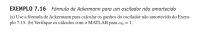
\includegraphics[width=1.2\linewidth]{./figs/Ex7.16}

Matriz de controlabilidade:
\begin{align}
 \mathcal{{C}} &= \begin{bmatrix} \mathbf{B} & | & \mathbf{AB}& \end{bmatrix} = \left[\begin{matrix}0 & 1\\1 & 0\end{matrix}\right] 
\end{align}

Inversa:
\begin{align}
\mathcal{{C}}^{-1} &= \left[\begin{matrix}0 & 1\\1 & 0\end{matrix}\right]
\end{align}

Note que, neste caso, a inversa é a própria matriz.

Matriz \(\mathbf{A}\) aplicada ao polinômio \(\alpha\):
\[
  \alpha(\mathbf{A}) = 4\omega_0^2\mathbf{I} + 4\omega_0 \mathbf{A} + \mathbf{A}^2 = \left[\begin{matrix}3 \omega_{0}^{2} & 4 \omega_{0}\\- 4 \omega_{0}^{3} & 3 \omega_{0}^{2}\end{matrix}\right]
\]

Fórmula de Ackerman:
\begin{align}
  \mathbf{K} = \begin{bmatrix} 0 & 1 \end{bmatrix} \, \left[\begin{matrix}0 & 1\\1 & 0\end{matrix}\right] \, \left[\begin{matrix}3 \omega_{0}^{2} & 4 \omega_{0}\\- 4 \omega_{0}^{3} & 3 \omega_{0}^{2}\end{matrix}\right] = \left[\begin{matrix}3 \omega_{0}^{2} & 4 \omega_{0}\end{matrix}\right]
\end{align}

Solução numérica com Python:

\begin{Shaded}
\begin{Highlighting}[]
\ImportTok{import}\NormalTok{ control }\ImportTok{as}\NormalTok{ ct}
\ImportTok{import}\NormalTok{ numpy }\ImportTok{as}\NormalTok{ np}

\NormalTok{w0 }\OperatorTok{=} \DecValTok{1}
\NormalTok{A }\OperatorTok{=}\NormalTok{ np.array([[}\DecValTok{0}\NormalTok{, }\DecValTok{1}\NormalTok{],[}\OperatorTok{{-}}\NormalTok{w0}\OperatorTok{**}\DecValTok{2}\NormalTok{, }\DecValTok{0}\NormalTok{]])}
\NormalTok{B }\OperatorTok{=}\NormalTok{ np.array([[}\DecValTok{0}\NormalTok{],[}\DecValTok{1}\NormalTok{]])}
\NormalTok{polos }\OperatorTok{=}\NormalTok{ [}\OperatorTok{{-}}\DecValTok{2}\OperatorTok{*}\NormalTok{w0, }\OperatorTok{{-}}\DecValTok{2}\OperatorTok{*}\NormalTok{w0]}
\NormalTok{K }\OperatorTok{=}\NormalTok{ ct.acker(A,B, polos)}
\BuiltInTok{print}\NormalTok{(K)}
\end{Highlighting}
\end{Shaded}

\begin{verbatim}
## [[3. 4.]]
\end{verbatim}

A fórmula de Ackermann permite posicionar os pólos de malha
fechada \textbf{em qualquer lugar desejado}, desde que a matriz de controlabilidade possua inversa.

Isso torna o projeto mais direto, comparado por exemplo, ao método de projeto com LGR, onde o posicionamento dos pólos com controle proporcional fica restrito ao lugar geométrico.

No entanto, isso é possível devido à hipótese forte de que todos os
estados estão disponíveis para realimentação.

\textbf{Exercício}

Use Ackermann para projetar um controlador para o sistema
\begin{align}
    G(s) &= \frac{30}{s(s+1)^2}
\end{align}

Posicione os pólos em \(-4\pm j4\) e \(-12\).

\hypertarget{introduuxe7uxe3o-da-referuxeancia}{%
\section{Introdução da referência}\label{introduuxe7uxe3o-da-referuxeancia}}

Até agora vimos como resolver o problema da regulação de estados apenas
para zerar o estado final. No entanto, o objetivo do controle é fazer a
saída rastrear a referência \(r\).

Uma forma simples de fazer isso é usando o sinal de controle:
\begin{align*}
u &= -\mathbf{Kx}+Nr
\end{align*}
onde \(\mathbf{K}\) é o vetor de ganhos conforme já definimos e \(N\) é
um ganho a se determinar.

Se usarmos esta lei de controle, a equação de estados do sistema em
malha fechada fica:

\[
\dot{\mathbf{x}} = \mathbf{(A-BK)x} + \mathbf{B}N\,r
\]

A equação de saída fica:
\[
y = (\mathbf{C}-D\mathbf{K})\mathbf{x}+DN\,r
\]

A função de transferência do sistema da entrada de referência \(r\) para a
saída \(y\) é:

\[
  G(s) = (\mathbf{C}-D\mathbf{K})(s\mathbf{I-A+BK})^{-1}\mathbf{B}N+DN
\]

Se quisermos que o sistema rastreie a referência em regime
permanente, \(y=r\), o ganho DC do sistema deve ser unitário, isto é,
\(G(0)=1\). Então fazemos \(G(0)=1\) na equação e resolvemos para \(N\). O
resultado é:

\[
  N = \frac{1}{(\mathbf{C}-D\mathbf{K})(\mathbf{-A+BK})^{-1}\mathbf{B}+D}
\]

Como normalmente o ganho \(D\) é nulo, temos o resultado mais usual:

\[
  N = \frac{1}{\mathbf{C}(\mathbf{-A+BK})^{-1}\mathbf{B}}
\]

O algoritmo de projeto é, portanto:

\begin{itemize}
\tightlist
\item
  Calcule o vetor de ganhos \(\mathbf{K}\) normalmente, conforme as
  especificações de projeto
\item
  Use o vetor \(\mathbf{K}\) calculado para determinar \(N\)
\item
  Implemente o algoritmo de controle como: \(u=-\mathbf{KX}+Nr\)
\end{itemize}

\includesvg{./figs/Ex.7.18.svg}
Precisamos apenas usar a expressão:
\[
  N = \frac{1}{\mathbf{C}(\mathbf{-A+BK})^{-1}\mathbf{B}}
\]
A saída do oscilador é a posição \(x_1\), logo \(\mathbf{C} = \begin{bmatrix}1 & 0\end{bmatrix}\). Usando o resultado anterior para \(\mathbf{K}\).

\begin{align}
  \mathbf{-A+BK} &= \left[\begin{matrix}0 & -1\\4 \omega_{0}^{2} & 4 \omega_{0}\end{matrix}\right] \\
  (\mathbf{-A+BK})^{-1} &= \left[\begin{matrix}\frac{1}{\omega_{0}} & \frac{1}{4 \omega_{0}^{2}}\\-1 & 0\end{matrix}\right]\\
  N &= \frac{1}{\mathbf{C}(\mathbf{-A+BK})^{-1}\mathbf{B}} &= \frac{1}{\frac{1}{4 \omega_{0}^{2}}} = 4 \omega_{0}^{2}
\end{align}

\hypertarget{simulauxe7uxe3o-em-malha-fechada}{%
\section{Simulação em malha fechada}\label{simulauxe7uxe3o-em-malha-fechada}}

É interessante testar o projeto agora usando uma resposta ao degrau. Note que para isso, precisamos definir o sistema em malha fechada.

Substituindo \(u=-\mathbf{Kx}+Nr\) na equação de estados vemos que as matrizes \(\mathbf{A}\) e \(\mathbf{B}\) em malha fechada mudam. A saída permanence a mesma, logo a matriz \(\mathbf{C}\) de malha fechada permanece a mesma.

Em malha fechada (i.e., ganhos realimentados), as equações do sistema ficam:
\begin{align}
    \mathbf{\dot{x}} &= \mathbf{(A-BK)x} +\mathbf{B}Nr\\
    y &= \mathbf{Cx}
\end{align}

A seguir resolvemos e simulamos o sistema do exemplo anterior com \(\omega_0=1\).

Imports e sistema

\begin{Shaded}
\begin{Highlighting}[]
\ImportTok{import}\NormalTok{ control }\ImportTok{as}\NormalTok{ ct}
\ImportTok{import}\NormalTok{ numpy }\ImportTok{as}\NormalTok{ np}

\NormalTok{w0 }\OperatorTok{=} \DecValTok{1}
\NormalTok{A }\OperatorTok{=}\NormalTok{ np.array([[}\DecValTok{0}\NormalTok{, }\DecValTok{1}\NormalTok{],[}\OperatorTok{{-}}\NormalTok{w0}\OperatorTok{**}\DecValTok{2}\NormalTok{, }\DecValTok{0}\NormalTok{]])}
\NormalTok{B }\OperatorTok{=}\NormalTok{ np.array([[}\DecValTok{0}\NormalTok{],[}\DecValTok{1}\NormalTok{]])}
\NormalTok{C }\OperatorTok{=}\NormalTok{ np.array([[}\DecValTok{1}\NormalTok{,}\DecValTok{0}\NormalTok{]])}
\end{Highlighting}
\end{Shaded}

Alocação de pólos e referência

\begin{Shaded}
\begin{Highlighting}[]
\NormalTok{polos }\OperatorTok{=}\NormalTok{ [}\OperatorTok{{-}}\DecValTok{2}\OperatorTok{*}\NormalTok{w0, }\OperatorTok{{-}}\DecValTok{2}\OperatorTok{*}\NormalTok{w0]}
\NormalTok{K }\OperatorTok{=}\NormalTok{ ct.acker(A,B, polos)}

\NormalTok{N }\OperatorTok{=} \DecValTok{1}\OperatorTok{/}\NormalTok{(C }\OperatorTok{@}\NormalTok{ np.linalg.inv(}\OperatorTok{{-}}\NormalTok{A}\OperatorTok{+}\NormalTok{B}\OperatorTok{@}\NormalTok{K) }\OperatorTok{@}\NormalTok{ B)}
\end{Highlighting}
\end{Shaded}

Matrizes de malha fechada. Repare o uso do símbolo @ para produto matricial.

\begin{Shaded}
\begin{Highlighting}[]
\NormalTok{Amf }\OperatorTok{=}\NormalTok{ A }\OperatorTok{{-}}\NormalTok{ B}\OperatorTok{@}\NormalTok{K}
\NormalTok{Bmf }\OperatorTok{=}\NormalTok{ B}\OperatorTok{@}\NormalTok{N}
\NormalTok{Cmf }\OperatorTok{=}\NormalTok{ C}
\NormalTok{Dmf }\OperatorTok{=}\NormalTok{ np.array([[}\DecValTok{0}\NormalTok{]])}

\CommentTok{\# Sistema}
\NormalTok{sis }\OperatorTok{=}\NormalTok{ ct.ss(Amf,Bmf,Cmf,Dmf)}
\end{Highlighting}
\end{Shaded}

Relatório de pólos de malha fechada

\begin{Shaded}
\begin{Highlighting}[]
\NormalTok{tab }\OperatorTok{=}\NormalTok{ ct.damp(sis)}
\end{Highlighting}
\end{Shaded}

\begin{verbatim}
##     Eigenvalue (pole)       Damping     Frequency
##                    -2             1             2
##                    -2             1             2
\end{verbatim}

Os pólos foram corretamente alocados. Repare que, por serem reais, o programa considera amortecimento (\emph{damping}) igual a 1 e a frequência natural é o módulo do pólo.

Zeros de transmissão

\begin{Shaded}
\begin{Highlighting}[]
\NormalTok{ct.zeros(sis)}
\end{Highlighting}
\end{Shaded}

\begin{verbatim}
## array([], dtype=complex128)
\end{verbatim}

O sistema não possui zeros.

Simula o sistema para uma resposta ao degrau unitário. Tempo de simulação é 7 segundos.

\begin{Shaded}
\begin{Highlighting}[]
\NormalTok{t,y }\OperatorTok{=}\NormalTok{ ct.step\_response(sis,}\DecValTok{7}\NormalTok{)}
\end{Highlighting}
\end{Shaded}

Plota os resultados, com algumas legendas

\begin{Shaded}
\begin{Highlighting}[]
\ImportTok{import}\NormalTok{ matplotlib.pyplot }\ImportTok{as}\NormalTok{ plt}
\NormalTok{plt.plot(t,y)}
\NormalTok{plt.grid()}
\NormalTok{plt.xlabel(}\StringTok{\textquotesingle{}Tempo (seg)\textquotesingle{}}\NormalTok{)}
\NormalTok{plt.ylabel(}\StringTok{\textquotesingle{}Saída\textquotesingle{}}\NormalTok{)}
\NormalTok{plt.legend(}\StringTok{\textquotesingle{}y\textquotesingle{}}\NormalTok{)}
\NormalTok{plt.show()}
\end{Highlighting}
\end{Shaded}

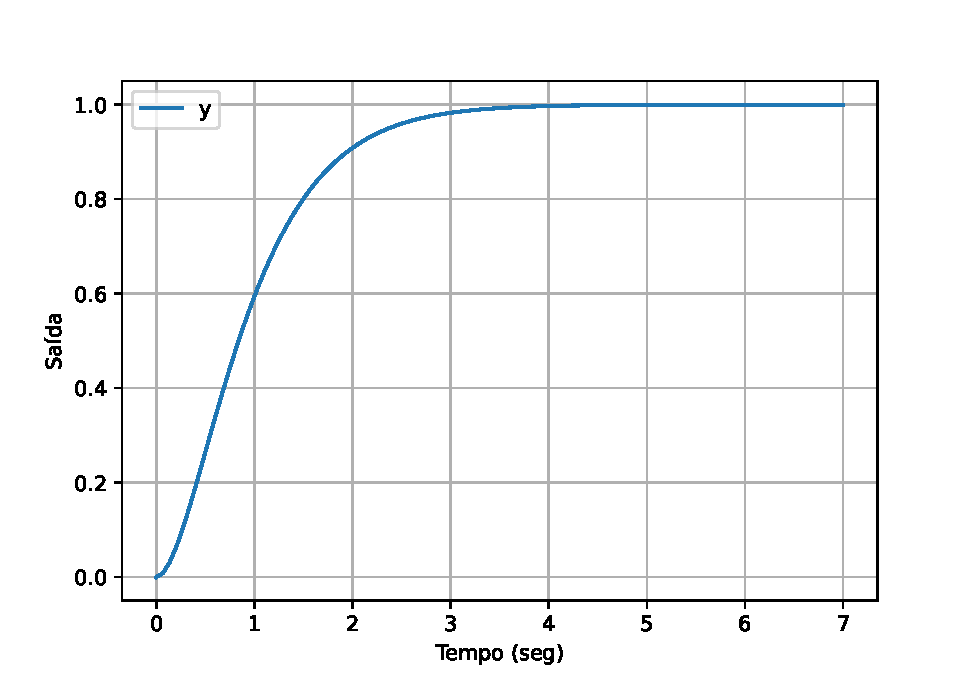
\includegraphics{_main_files/figure-latex/unnamed-chunk-34-1.pdf}

\hypertarget{escolha-dos-puxf3los}{%
\section{Escolha dos pólos}\label{escolha-dos-puxf3los}}

O sucesso do controle depende da escolha adequada do polinômio de malha fechada desejado. Esse polinômio deve ser construído tendo em mente todos os pólos de malha fechada desejados, não
apenas os dominantes.

Isso é importante quando temos um sistema de ordem maior que 2: os pólos que não serão dominantes devem ser escolhidos suficientemente distantes dos candidatos a dominantes.

Uma regra prática é, após escolher os dominantes, escolher os demais como reais, com a parte real de 3 a 5 vezes maior que a parte real dos dominantes.

Lembre-se, porém, que se o deslocamento dos polos para a nova posição for muito grande, os ganhos do controlador vão aumentar e consequentemente o sinal de controle vai exigir mais energia.

Outra coisa a se ter em mente na hora de escolher pólos de malha fechada são os zeros do sistema. \textbf{A realimentação de estados não altera a posição dos zeros}, isto é, se eles não forem cancelados, eles permanecerão na mesma posição em malha fechada. Agora, se estes zeros estiverem próximos dos pólos dominantes em malha fechada, a dinâmica projetada não irá funcionar corretamente (normalmente o overshoot será mais alto do que o projetado).

Uma forma de lidar com isso é posicionar um pólo extra sobre o zero que está atrapalhando o projeto, mas \textbf{apenas se o zero for estável}.

Note que devido às incertezas e os arredondamentos de projeto, podemos ter que fazer novas escolhas de polos até achar uma combinação que se ajuste ao que precisamos.

\includesvg{./figs/Ex7.20.svg}

Observe a solução com Python.

\begin{Shaded}
\begin{Highlighting}[]
\CommentTok{\# Imports}
\ImportTok{import}\NormalTok{ control }\ImportTok{as}\NormalTok{ ct}
\ImportTok{import}\NormalTok{ numpy }\ImportTok{as}\NormalTok{ np}

\CommentTok{\# Sistema}
\NormalTok{A }\OperatorTok{=}\NormalTok{ np.array([  [}\DecValTok{0}\NormalTok{, }\DecValTok{2}\NormalTok{, }\DecValTok{0}\NormalTok{, }\DecValTok{0}\NormalTok{, }\DecValTok{0}\NormalTok{],}
\NormalTok{                [}\OperatorTok{{-}}\FloatTok{.1}\NormalTok{, }\OperatorTok{{-}}\FloatTok{.35}\NormalTok{, }\FloatTok{.1}\NormalTok{, }\FloatTok{.1}\NormalTok{, }\FloatTok{.75}\NormalTok{], }
\NormalTok{                [}\DecValTok{0}\NormalTok{, }\DecValTok{0}\NormalTok{, }\DecValTok{0}\NormalTok{, }\DecValTok{2}\NormalTok{, }\DecValTok{0}\NormalTok{],}
\NormalTok{                [}\FloatTok{.4}\NormalTok{, }\FloatTok{.4}\NormalTok{, }\OperatorTok{{-}}\FloatTok{.4}\NormalTok{, }\OperatorTok{{-}}\FloatTok{1.4}\NormalTok{, }\DecValTok{0}\NormalTok{],}
\NormalTok{                [}\DecValTok{0}\NormalTok{, }\OperatorTok{{-}}\FloatTok{.03}\NormalTok{, }\DecValTok{0}\NormalTok{, }\DecValTok{0}\NormalTok{, }\OperatorTok{{-}}\DecValTok{1}\NormalTok{]     ],dtype}\OperatorTok{=}\BuiltInTok{float}\NormalTok{)}
\NormalTok{B }\OperatorTok{=}\NormalTok{ np.array([[}\DecValTok{0}\NormalTok{],[}\DecValTok{0}\NormalTok{],[}\DecValTok{0}\NormalTok{],[}\DecValTok{0}\NormalTok{],[}\DecValTok{1}\NormalTok{]])}
\NormalTok{C }\OperatorTok{=}\NormalTok{ np.array([[}\DecValTok{1}\NormalTok{,}\DecValTok{0}\NormalTok{,}\DecValTok{0}\NormalTok{,}\DecValTok{0}\NormalTok{,}\DecValTok{0}\NormalTok{]])}
\NormalTok{D }\OperatorTok{=}\NormalTok{ np.array([[}\DecValTok{0}\NormalTok{]])}
\end{Highlighting}
\end{Shaded}

Pólos desejados, calculados pelos parâmetros físicos

\begin{Shaded}
\begin{Highlighting}[]
\NormalTok{xi }\OperatorTok{=} \FloatTok{0.707}
\NormalTok{wn }\OperatorTok{=} \DecValTok{1}\OperatorTok{/}\FloatTok{1.15}
\NormalTok{p }\OperatorTok{=} \OperatorTok{{-}}\NormalTok{xi}\OperatorTok{*}\NormalTok{wn}\OperatorTok{+}\OtherTok{1j}\OperatorTok{*}\NormalTok{wn}\OperatorTok{*}\NormalTok{np.sqrt(}\DecValTok{1}\OperatorTok{{-}}\NormalTok{xi}\OperatorTok{**}\DecValTok{2}\NormalTok{)}
\end{Highlighting}
\end{Shaded}

Polos de malha fechada desejados, conjunto completo. Note a forma de gerar os pólos adicionais usando o dominante como referência e o recurso de repetição de elementos de uma lista.

\begin{Shaded}
\begin{Highlighting}[]
\NormalTok{polos\_dom }\OperatorTok{=}\NormalTok{ np.array([[p, np.conjugate(p)]])}
\NormalTok{polos\_extras }\OperatorTok{=}\NormalTok{ np.array([[np.real(p)}\OperatorTok{*}\DecValTok{4}\NormalTok{]}\OperatorTok{*}\DecValTok{3}\NormalTok{])}
\NormalTok{polos\_mf }\OperatorTok{=}\NormalTok{ np.block([polos\_dom,polos\_extras])}
\end{Highlighting}
\end{Shaded}

Alocação de polos e referência

\begin{Shaded}
\begin{Highlighting}[]
\NormalTok{K }\OperatorTok{=}\NormalTok{ ct.acker(A,B,polos\_mf[}\DecValTok{0}\NormalTok{,:])}
\NormalTok{N }\OperatorTok{=} \DecValTok{1}\OperatorTok{/}\NormalTok{(C }\OperatorTok{@}\NormalTok{ np.linalg.inv(}\OperatorTok{{-}}\NormalTok{A}\OperatorTok{+}\NormalTok{B}\OperatorTok{@}\NormalTok{K) }\OperatorTok{@}\NormalTok{ B)}
\end{Highlighting}
\end{Shaded}

O vetor de ganhos encontrado é \(\mathbf{K} = \left[\begin{matrix}8.1 & 19.33 & 1.27 & -0.2139 & 5.857\end{matrix}\right]\)

\textbf{Os valores são um pouco diferentes do livro. Tente descobrir a razão}

Simulação em malha fechada:

\begin{Shaded}
\begin{Highlighting}[]
\NormalTok{Amf }\OperatorTok{=}\NormalTok{ A }\OperatorTok{{-}}\NormalTok{ B}\OperatorTok{@}\NormalTok{K}
\NormalTok{Bmf }\OperatorTok{=}\NormalTok{ B}\OperatorTok{@}\NormalTok{N}
\NormalTok{Cmf }\OperatorTok{=}\NormalTok{ C}
\NormalTok{Dmf }\OperatorTok{=}\NormalTok{ np.array([[}\DecValTok{0}\NormalTok{]])}

\CommentTok{\# Sistema}
\NormalTok{sis }\OperatorTok{=}\NormalTok{ ct.ss(Amf,Bmf,Cmf,Dmf)}

\CommentTok{\# Simulação}
\NormalTok{t,y }\OperatorTok{=}\NormalTok{ ct.step\_response(sis,}\DecValTok{7}\NormalTok{)}

\NormalTok{plt.plot(t,y)}
\NormalTok{plt.grid()}
\NormalTok{plt.xlabel(}\StringTok{\textquotesingle{}Tempo (seg)\textquotesingle{}}\NormalTok{)}
\NormalTok{plt.ylabel(}\StringTok{\textquotesingle{}Saída\textquotesingle{}}\NormalTok{)}
\NormalTok{plt.legend(}\StringTok{\textquotesingle{}y\textquotesingle{}}\NormalTok{)}
\NormalTok{plt.show()}
\end{Highlighting}
\end{Shaded}

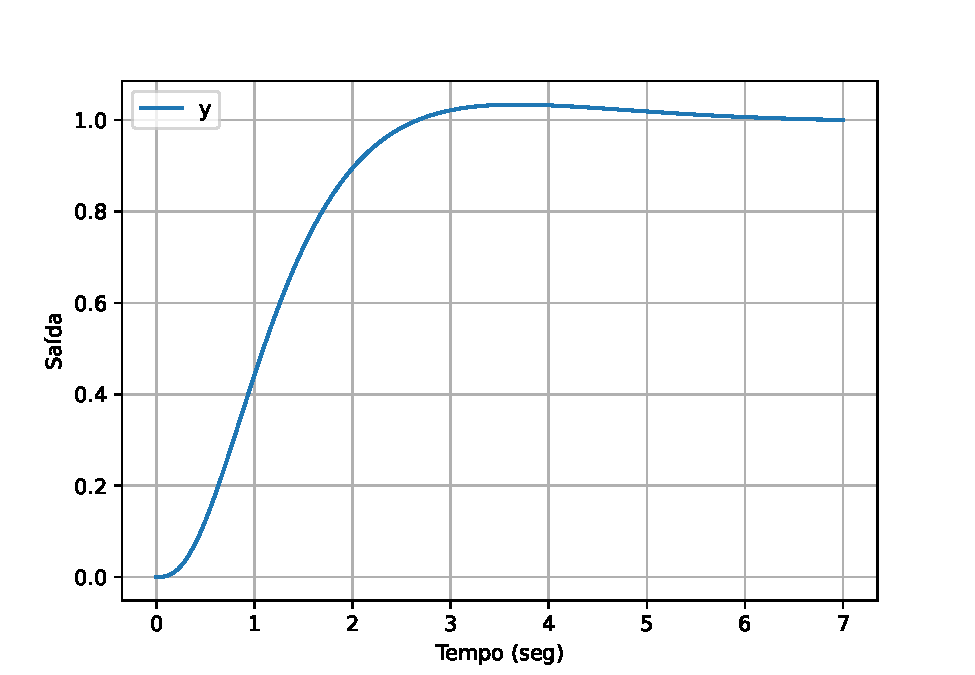
\includegraphics{_main_files/figure-latex/unnamed-chunk-40-3.pdf}

É sempre importante analisar as características do sistema (pólos e zeros), além dos sinais.

\begin{Shaded}
\begin{Highlighting}[]
\NormalTok{tab }\OperatorTok{=}\NormalTok{ ct.damp(sis)}
\end{Highlighting}
\end{Shaded}

\begin{verbatim}
##     Eigenvalue (pole)       Damping     Frequency
##                -2.459             1         2.459
##     -2.459+2.019e-05j             1         2.459
##     -2.459-2.019e-05j             1         2.459
##    -0.6148    +0.615j         0.707        0.8696
##    -0.6148    -0.615j         0.707        0.8696
\end{verbatim}

Zeros:

\begin{Shaded}
\begin{Highlighting}[]
\NormalTok{sis.zeros()}
\end{Highlighting}
\end{Shaded}

\begin{verbatim}
## array([-0.7+0.55677644j, -0.7-0.55677644j])
\end{verbatim}

valor máximo de saída:

\begin{Shaded}
\begin{Highlighting}[]
\BuiltInTok{print}\NormalTok{(}\BuiltInTok{max}\NormalTok{(y))}
\end{Highlighting}
\end{Shaded}

\begin{verbatim}
## 1.0339565325466082
\end{verbatim}

Tente explicar o que aconteceu com o projeto em malha fechada. Faça correlação com o gráfico do sinal de saída.

\textbf{Exemplo:}

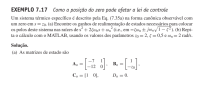
\includegraphics[width=1\linewidth]{./figs/Ex7.17}

Abaixo apenas o item (b), resolvendo direto com acker()

Execute novamente o código com \(z_0=3\) para verificar a variação dos
ganhos como no livro. Espera-se que haja um aumento significativo nos
ganhos.

Quando um polo e um zero tendem a se cancelar, o sistema tende a perder
controlabilidade e isso torna os ganhos mais altos e, consequentemente,
o controle fica mais ``caro'' (puxa mais energia). Vale a observação do
livro:

\textbf{``O sistema tem que trabalhar com mais força para conseguir o controle
quando a controlabilidade é fraca.''}

Além disso:

\textbf{``Mover os polos em um longo caminho requer grandes ganhos.''}

Isso é observado quando um sistema é naturalmente lento e tentamos
deixá-lo mais rápido. Isso normalmente resulta em ganhos grandes (em
módulo), o que resulta novamente em um controle ``caro''.

\hypertarget{estimadores-de-estado}{%
\section{Estimadores de estado}\label{estimadores-de-estado}}

No assunto anterior vimos que a ação de controle no espaço de estados é
proporcional aos estados do sistema. Para isso ser possível de calcular,
precisamos ter esses sinais disponíveis.

Na prática, uma medição direta dos estados é raramente viável. O número
de sensores pode ser grande, o que tornaria o projeto muito caro. Ou
simplesmente, os estados não são possíveis de medir.

Para contornar a situação usamos um sistema auxiliar, um subsistema do
controlador, que é responsável por fornecer uma estimativa dos estados
reais. Esse sistema é chamado de \textbf{estimador} ou \textbf{observador de
estados}.

\hypertarget{modelagem-do-observador}{%
\section{Modelagem do observador}\label{modelagem-do-observador}}

Vamos supor que os estados reais sejam \(\mathbf{x}\) e a respectiva
estimativa seja \(\hat{\mathbf{x}}\). Idealmente, queremos que
\(\hat{\mathbf{x}}\approx \mathbf{x}\).

Suponha que o sistema real seja: \[
\begin{align*}
    \dot{\mathbf{x}} &= \mathbf{Ax+B}u\\
    y &= \mathbf{Cx} + Du
\end{align*}
\]

O estimador é um sistema que tenta ``imitar'' o original, usando uma
dinâmica parecida: \[
\begin{align*}
    \dot{\mathbf{\hat{x}}} &= \mathbf{A\hat{x}+B}u+\mathbf{L}(y-\mathbf{C\hat{x}})
\end{align*}
\]

A interpretação dessa equação é a seguinte:

\begin{itemize}
\tightlist
\item
  O termo \(\mathbf{A\hat{x}+B}u\) é uma tentativa de ``imitar'' a equação
  original do sistema.
\item
  O termo \(\mathbf{L}(y-\mathbf{C\hat{x}})\) é um fator de correção do
  anterior.

  \begin{itemize}
  \tightlist
  \item
    O termo \(\mathbf{C\hat{x}}\) representa uma estimativa da saída
    do sistema (é a matriz de saída \(\mathbf{C}\) vezes os estados
    estimados)
  \item
    O termo \(y-\mathbf{C\hat{x}}\) representa, portanto, o erro entre
    a saída real e a saída estimada.
  \item
    O vetor coluna \(\mathbf{L}\) funciona como um ganho proporcional.
  \end{itemize}
\end{itemize}

Assim, vemos que o estimador é um sistema que ``imita'' a dinâmica do
sistema original, porém, ele corrige o erro da dinâmica usando uma
parcela proporcional ao erro de estimativa da saída (que é um sinal que
nós realmente conseguimos medir).

Esse termo de correção é o que faz o estimador funcionar. Projetar o
estimador é essencialmente calcular o vetor \(\mathbf{L}\), chamado de
\emph{ganho do estimador}.

Se o ganho do estimador for bem projetado, a diferença entre
\(\mathbf{x}-\mathbf{\hat{x}}\) cairá rapidamente com o tempo. Ou seja,
passado um longo tempo (isto é, em regime permanente), \(\mathbf{x}\) e
\(\mathbf{\hat{x}}\) terão os mesmos valores. Matematicamente
representamos \(\mathbf{x}\rightarrow \mathbf{\hat{x}}\).

\includesvg{./figs/Fig7.28.svg}

A síntese do estimador é feita da seguinte maneira. Seja
\(e = \mathbf{x}-\mathbf{\hat{x}}\) o erro de estimação entre os estados.
Combinando a dinâmica do sistema e do estimador, podemos mostrar que: \[
\begin{align*}
    \dot{\mathbf{e}} &= \mathbf{(A-LC)e}
\end{align*}
\]

Esse é um sistema autônomo (sem entrada), que só depende das condições
iniciais. Ele só possui a matriz de estados, que se for estável, fará
com que o estado inicial decaia a zero, qualquer que ele seja.

Em outras palavras, mesmo que não conheçamos o estado inicial do sistema
para alimentar o estimador, o erro ainda assim irá para zero em regime
permanente.

Para que isso aconteça, basta que a matriz \(\mathbf{(A-LC)}\) seja
estável, isto é, tenha todos os autovalores no SPE.

Esse é um problema semelhante ao da regulação de estados. A única
diferença é a posição das matrizes. No problema de regulação temos
\(\mathbf{A-BK}\).

\begin{longtable}[]{@{}lcc@{}}
\toprule\noalign{}
& Regulador & Estimador \\
\midrule\noalign{}
\endhead
\bottomrule\noalign{}
\endlastfoot
Determinar & \(\mathbf{K}\) & \(\mathbf{L}\) \\
Dimensões & \(1\times n\) & \(n\times 1\) \\
Equação & \(\mathbf{F-GK}\) & \(\mathbf{F-LH}\) \\
\end{longtable}

Devido às semelhanças, podemos usar as mesmas estratégias e funções
Python para projetar o estimador.

\textbf{Exemplo:}

\includesvg{./figs/Ex7.25.svg}

\textbf{Solução numérica}

Se adotarmos \(\omega_0=1\), podemos resolver o mesmo problema usando a
função de posicionamento de polos \emph{acker()}. De fato, isso é possível,
porque o problema do observador é muito semelhante ao do regulador,
mudando apenas os seguintes parâmetros. * Usamos \(\mathbf{F}^T\) ao
invés de \(\mathbf{F}\) * Usamos \(\mathbf{H}^T\) ao invés de \(\mathbf{G}\)
* Transpomos o resultado para obter o ganho do observador na forma de
vetor coluna

\hypertarget{forma-canuxf4nica-de-observador-e-observabilidade}{%
\section{Forma canônica de observador e observabilidade}\label{forma-canuxf4nica-de-observador-e-observabilidade}}

Tal como no caso do regulador de estados, há uma forma de espaço de
estados para a qual a solução do observador é muito simples. A forma é
conhecida como forma canônica de observador.

Para deduzi-la procedemos como anteriormente. Desenhamos um diagrama de
blocos e extraimos as equações de estados dos integradores.

O caso de terceira ordem geral é mostrado na Figura abaixo.

\includesvg{./figs/Fig7.31.svg}

A função de transferência correspondente é: \[
\begin{align*}
    G(s) = \frac{b_1s^2+b_2s+b_3}{s^3+a_1s^2+a_2s+a_3}
\end{align*}
\]

Note que:

\begin{itemize}
\tightlist
\item
  Os integradores \textbf{não} estão em série diretamente
\item
  Entre cada integrador há um somador
\item
  Apenas a saída (último integrador) é realimentada
\item
  A realimentação é feita para cada um dos somadores, através dos
  ganhos do denominador
\item
  A entrada se conecta a cada um dos somadores, através dos ganhos do
  numerador
\end{itemize}

A representação de estados é:

\[
\begin{align*}
    \mathbf{\dot{x}} &= \left[
        \begin{array}{rrr}
        -a_1 & 1 & 0\\
        -a_2 & 0 & 1\\
        -a_3 & 0 & 0\end{array}
    \right]\mathbf{{x}}+
    \left[\begin{array}{rrr}
        b_1\\
        b_2\\
        b_3\end{array}
    \right]u\\
    y &= \left[\begin{array}{ccc} 1 & 0 & 0\end{array}\right]\mathbf{x}
\end{align*}
\]

Note que: * Na matriz \(\mathbf{A}\), a primeira coluna é formada pelos
coeficientes do denominador com sinal trocado, ordem crescente de
potência de \(s\), de cima para baixo. * As colunas restantes podem ser
montadas usando uma matriz identidade de ordem 2 e uma linha de zeros *
A matriz \(\mathbf{B}\) é uma coluna formada pelos coeficientes do
numerador, ordem crescente de potência de \(s\) de cima para baixo. * A
matriz \(\mathbf{C}\) é uma linha de zeros, exceto pelo primeiro elemento
igual a 1. * \(J=0\).

\textbf{Exercício:} Desenhe e obtenha as matrizes para o caso de 4a ordem.

A forma de observador é útil no projeto de observadores. Para o caso de
3a ordem anterior, a matriz de projeto é \[
\begin{align*}
\mathbf{A-LC} &= \left[
        \begin{array}{rrr}
        -a_1-l_1 & 1 & 0\\
        -a_2-l_2 & 0 & 1\\
        -a_3-l_3 & 0 & 0\end{array}
    \right]
\end{align*}
\] cuja equação característica é: \[
\begin{align*}
s^3+(a_1+l_1)s^2+(a_2+l_2)s+(a_3+l_3)=0
\end{align*}
\]

Assim, podemos achar os ganhos do observador
\(\mathbf{L}=\left[\begin{array}{ccc} l_1 & l_2 & l_3\end{array} \right]\)
muito facilmente com o polinômio desejado.

\hypertarget{observabilidade}{%
\subsection{Observabilidade}\label{observabilidade}}

Observabilidade é a capacidade que um sistema possui em ``permitir'' que
seus estados sejam estimados a partir apenas do conhecimento do sinal de
saída.

Da mesma forma que a controlabilidade, podemos medir a observabilidade
pela \textbf{matriz de observabilidade} e seu determinante.

A matriz de observabilidade é construída linha por linha, como: \[
\begin{align*}
\mathbf{\mathcal{O}} &= \left[
        \begin{array}{c}
        \mathbf{C}\\
        \mathbf{CA}\\
        \mathbf{CA^2}\\
        \vdots\\
        \mathbf{CA^{n-1}}
        \end{array}
    \right]
\end{align*}
\]

Uma forma rápida de calcular essa matriz é usar a função obsv() da
biblioteca \emph{control}.

Um sistema SISO é observável se \(\det \mathbf{\mathcal{O}} \neq 0\). Se o
sistema é MIMO, devemos olhar para o posto da matriz de observabilidade.

O sistema perde observabilidade quando há cancelamentos entre pólos
zeros, de forma semalhante à controlabilidade. O sistema torna-se mais
observável à medida que possui mais saídas mensuráveis.

Observe que existem diversos paralelos entre controlabilidade e
observabilidade, inclusive nos cálculos.

Como já mostramos, os cálculos de observabilidades basicamente trocam a
matriz \(\mathbf{B}\) pela transposta de \(\mathbf{C}\) e a matriz de
estados pela sua transposta. Esse ``paralelismo'' é chamado de \emph{dualidade}
entre as duas propriedades.

\hypertarget{estimador-de-ordem-reduzida}{%
\subsection{Estimador de ordem reduzida}\label{estimador-de-ordem-reduzida}}

O estimador de estados como apresentado reconstrói o vetor de estados
original completamente. No entanto, em muitas situações, um dos estados
reconstruídos é o próprio sinal de saída, que é diretamente mensurável.

Alguns projetistas consideram isso um ``desperdício'' de recursos. Por
esse motivo, existe o projeto do estimador de ordem reduzida.

A redução de ordem é igual ao número de saídas medidas do sistema. No
nosso caso, que só trabalhamos com SISO, a redução é de apenas 1
unidade. Mas a ideia é aplicável a casos MIMO também, o que pode ser
bastante útil dependendo do sistema.

O estimador reduzido funciona muito parecido com o estimador completo.
Ele consiste de um ganho constante \(\mathbf{L}_t\), que é a solução do
problema de alocação de pólos: \[
\begin{align*}
    \det \left(s\mathbf{I-}\mathbf{A}_{bb}+\mathbf{L}\mathbf{A}_{ab}\right) = 0
\end{align*}
\]

onde as matrizes \(\mathbf{A}_{bb}\) e \(\mathbf{A}_{ab}\) são obtidas
diretamente da matriz \(\mathbf{F}\) do sistema (preferencialmente em
forma de observador) através de particionamento.

Supondo o sistema em forma canônica de observador, em que a \textbf{saída é
exatamente igual ao primeiro estado}, isto é:
\(\mathbf{C}=\left[\begin{array}{cccc}1 & 0 & \ldots & 0\end{array}\right]\),
então fazemos o seguinte particionamento da matriz \(\mathbf{F}\) para
encontrar as matrizes de projeto do observador reduzido: \[
\begin{align*}
\mathbf{A} &= \left[
\begin{array}{cc}
    {A}_{aa} & \mathbf{A}_{ab}\\
    \mathbf{A}_{ba} & \mathbf{A}_{bb}\\
\end{array}
\right]
\end{align*}
\]

Note que: * \(A_{aa}\) é um escalar (apenas em sistemas SISO) *
\(\mathbf{A}_{ab}\) é uma linha * \(\mathbf{A}_{ba}\) é uma coluna *
\(\mathbf{A}_{bb}\) é quadrada, de ordem \(n-1\)

Basta então particionar a matriz \(\mathbf{A}\) no primeiro elemento da
primeira linha e coluna.

Por exemplo, para o caso de terceira ordem: \[
\begin{align*}
\mathbf{A} &= \left[
        \begin{array}{rrr}
        -a_1 & 1 & 0\\
        -a_2 & 0 & 1\\
        -a_3 & 0 & 0\end{array}
    \right]
\end{align*}
\]

Temos: \[
\begin{align*}
\mathbf{A}_{bb} &= \left[
        \begin{array}{rrr}
         0 & 1\\
         0 & 0\end{array}
    \right]\\
\mathbf{A}_{ab} &= \left[
        \begin{array}{rrr}
         1 & 0\end{array}
    \right]    
\end{align*}
\]

A figura abaixo ilustra os fluxos de sinal para implementação de um
observador reduzido.

\includesvg{./figs/Fig7.32.svg}

\hypertarget{compensador-dinuxe2mico}{%
\section{Compensador dinâmico}\label{compensador-dinuxe2mico}}

Já aprendemos a projetar um regulador, que é um conjunto de ganhos que
calcula a ação de controle usando os estados do sistema.

Também aprendemos a projetar um observador de estados, que é um sistema
dinâmico cuja função é fornecer uma estimativa dos estados reais do
sistema a partir do sinal de saída.

O compensador dinâmico é a junção destas duas ideias no mesmo sistema.

A Figura abaixo esquematiza todos os subsistemas e rotas de sinal com a
estratégia adotada.

\includesvg{./figs/Fig7.35.svg}

No final, nosso controlador projetado com essas abordagens é um único
sistema, cujas equações de estado são: \[ 
\begin{align*}
    \dot{\mathbf{x}}_e &= \mathbf{(A-BK-LC)}\mathbf{x}_e+\mathbf{L}y\\
    u &= \mathbf{-K}\mathbf{x}_e
\end{align*}
\] onde \(\mathbf{x}_e\) é a estimativa dos estados do sistema pelo
observador, \(\mathbf{K}\) e \(\mathbf{L}\) são respectivamente os ganhos do
regulador e do observador. Note que a entrada do controlador é a saída
da planta. Da mesma forma, o sinal de saída do controlador é o sinal de
controle \(u\), que vai para a entrada da planta.

Perceba, que estas duas equações permitem realizar o controlador como um
sistema entrada-saída normal, com uma função de transferência que
basicamente dispensa as equações de estado, para fins de implementação.
Esta função é: \[ 
\begin{align*}
    Q(s) &= -\mathbf{K}(s\mathbf{I-A+BK+LC})^{-1}\mathbf{L}
\end{align*}
\]

Para fins de simulação, o sistema completo (planta+controlador) podem
ser simulados usando um único conjunto de equações de estados: \[
\begin{align*}
\dot{\mathbf{x}} &= \mathbf{A}\mathbf{x}-\mathbf{BK}\mathbf{x_e}\\
\dot{\mathbf{x}}_e &= \mathbf{(A-BK-LC)}\mathbf{x}_e+\mathbf{LCx}\\
y&= \mathbf{Cx}
\end{align*}
\]

É possível demonstrar que os pólos de malha fechada compensado por um
controlador dessa natureza são exatamente os pólos projetados pelo
regulador de estados completo (isto é, considerando realimentação dos
estados verdadeiros, mesmo que na prática não vá ser assim no final) e o
pólos alocados para o observador.

Em outras palavras, o polinômio de malha fechada quando usamos um
compensador que combina regulador+observador é simplesmente: \[
\begin{align*}
    \alpha_{\text{mf}}(s) = \alpha_{\text{reg}}(s)\cdot \alpha_{\text{obs}}(s)
\end{align*}
\] onde ``mf'', ``reg'' e ``obs'' indicam respectivamente ``malha fechada'',
``regulador'' e ``observador''.

O fato do projeto dos dois sistemas não ``misturar'' os pólos é um fato
notável, que permite que os projetos sejam feitos de forma independente.
Isso é chamado de principío da separação em teoria de controle.

\hypertarget{implementauxe7uxe3o-quando-o-observador-uxe9-reduzido}{%
\subsection{Implementação quando o observador é reduzido}\label{implementauxe7uxe3o-quando-o-observador-uxe9-reduzido}}

Quando o observador usado é de ordem reduzida, as equações de estado do
controlador sofrem algumas mudanças, para acomodar a suposição que um
dos estados é medido e o particionamento de matrizes.

A função de transferência com o observador reduzido é: \[
\begin{align*}
Q(s) &= \mathbf{C}_r(s\mathbf{I}-\mathbf{A}_r)^{-1}\mathbf{B}_r+D_r
\end{align*}
\] onde: \[
\begin{align*}
\mathbf{A}_r &= \mathbf{A}_{bb}-\mathbf{LA}_{ab}-(\mathbf{B}_{b}-\mathbf{LB}_{a})\mathbf{K}_b\\
\mathbf{B}_r &= \mathbf{A}_{r}\mathbf{L}+\mathbf{A}_{ba}-\mathbf{L}\mathbf{A}_{aa}-(\mathbf{B}_{b}-\mathbf{LC}_{a}){K}_a\\
\mathbf{C}_r &= -\mathbf{K}_b\\
D_r &= -K_a-\mathbf{K}_b\mathbf{L}
\end{align*}
\]

No caso, as matrizes \(\mathbf{A}_{aa}\), \(\mathbf{A}_{ab}\),
\(\mathbf{A}_{ba}\), \(\mathbf{A}_{a}\) e \(\mathbf{A}_{b}\) são provenientes
do particionamento das matrizes do sistema, conforme o projeto do
observador reduzido.

A matriz \(\mathbf{K}_{b}\) e o ganho \({K}_{a}\) são provenientes do
particionamento do vetor de ganhos do regulador. O ganho \(K_a\) é o ganho
associado ao estado diretamente medido (i.e.~a saída) e \(\mathbf{K}_{b}\)
é o restante do vetor projetado.

\includesvg{./figs/Ex7.28.svg}

Vamos resolver usando as funções diretas de alocação de polos

\includesvg{./figs/Ex7.30.svg}

\hypertarget{introduuxe7uxe3o-da-referuxeancia-e-controle-integral}{%
\section{Introdução da referência e controle integral}\label{introduuxe7uxe3o-da-referuxeancia-e-controle-integral}}

Sabemos que um integrador em malha aberta zera o erro de regime
permanente (para uma entrada degrau pelo menos) e permite ao sistema
rejeitar distúrbios (do tipo degrau). Portanto, a introdução de
integradores na malha aberta é um aspecto desejável do projeto.

Para introduzir um integrador no espaço de estados, adicionamos um novo
estado ao sistema, que representa a integral do erro à referência: \[
\begin{align*}
    {e} = \int (r-y)dt
\end{align*}
\]

Supondo que \(y=\mathbf{Cx}\), a equação de estado deste novo sinal é: \[
\begin{align*}
    \dot{e} = r-\mathbf{Cx}
\end{align*}
\]

Essa última equação aumenta a ordem do sistema em 1. O sistema em malha
aberta agora fica: \[
\begin{align*}
    \dot{\mathbf{x}} &= \mathbf{Ax}+\mathbf{B}u\\
    \dot{e} &= r-\mathbf{Cx}
\end{align*}
\]

Em notação matricial em blocos temos: \[
\begin{align*}
    \left[\begin{array}{c}\dot{\mathbf{x}}\\ \dot{e}\end{array}\right]&=
    \left[\begin{array}{cc}\mathbf{A} & \mathbf{0}\\-\mathbf{C} & 0\end{array}\right]\left[\begin{array}{c}{\mathbf{x}}\\ {e}\end{array}\right]+\left[\begin{array}{c}\mathbf{B}\\ 0\end{array}\right]u+\left[\begin{array}{c}\mathbf{0}\\ 1\end{array}\right]r
\end{align*}
\]

Dizemos que o sistema está \emph{aumentado}

O algoritmo de controle integral consiste em fazer uma realimentação
completa de todos os estados agora definidos. \[
\begin{align*}
    u = -\mathbf{K}_a\mathbf{x}_a
\end{align*}
\]

Algoritmo de projeto:

\begin{itemize}
\item
  Construa as matrizes aumentadas: \[
  \begin{align*}
  \mathbf{A}_a &= \left[\begin{array}{cc}\mathbf{A} & \mathbf{0}\\-\mathbf{C} & 0\end{array}\right]\\
  \mathbf{B}_a &=\left[\begin{array}{c}\mathbf{B}\\ 0\end{array}\right]
  \end{align*}
  \]
\item
  Resolva o problema de regulação com
  \((\mathbf{A}_a, \, \mathbf{B}_a)\), para encontrar a matriz de ganhos
  aumentada \(\mathbf{K}_a\)
\end{itemize}

\hypertarget{escolha-dos-puxf3los-1}{%
\subsection{Escolha dos pólos}\label{escolha-dos-puxf3los-1}}

Perceba que a introdução de um integrador aumenta a ordem do sistema e
isso vai requerer a especificação de pólos adicionais. Tente alocar
estes pólos em posições estratégicas para não comprometer a dominância
dos pólos desejados.

\hypertarget{equauxe7uxf5es-de-estado-do-compensador}{%
\subsection{Equações de estado do compensador:}\label{equauxe7uxf5es-de-estado-do-compensador}}

No controle integral, projetamos o observador de estados normalmente,
como se o integrador não estivesse presente.

Supondo que os estados do observador são \(\mathbf{z}=\hat{\mathbf{x}}\),
as equações do compensador serão:

\[ 
\begin{align*}
    \dot{\mathbf{z}}&= (\mathbf{A}'-\mathbf{B}'\mathbf{K}_a-\mathbf{L}_0\mathbf{C}')\mathbf{z}+\mathbf{L}_1y+\mathbf{M}r\\
    u &= \mathbf{-K}_a\mathbf{z}
\end{align*}
\]

As matrizes aumentadas são:

\begin{align}
\mathbf{A}' &= \left[\begin{array}{ll}
                     \mathbf{A} & \mathbf{0}_{n\times 1}\\
                     \mathbf{0}_{1\times n} & 0
                \end{array}\right]\\

\mathbf{B}' &= \left[\begin{array}{cc}
\mathbf{B} \\ {0}
\end{array}\right]\\

\mathbf{C}' &= \left[\begin{array}{cc}
\mathbf{C} & {0}
\end{array}\right]\\

\mathbf{L}_0 &= \left[\begin{array}{cc}
\mathbf{L} \\ {0}
\end{array}\right]\\

\mathbf{L}_1 &= \left[\begin{array}{rr}
\mathbf{L} \\ {-1}
\end{array}\right]\\

\mathbf{M} &= \left[\begin{array}{cc}
\mathbf{0}_{n\times 1} \\ 1
\end{array}\right]
\end{align}

É interessante observar que esse compensador requer duas entradas
distintas para ser realizado: a referência e a saída da planta.

Lembre-se que do ponto de vista do controlador, a saída é o sinal de
controle \(u\). Portanto, a saída da planta \(y\) é vista por ele como uma
entrada, assim como a referência \(r\).

Podemos enxergá-lo através de duas funções de transferência: uma de \(Y\)
para \(U\) e outra de \(R\) para \(U\). Assim, a saída do controlador poderia
ser descrita como:

\begin{align}
    U(s) = C_1(s)Y(s)+C_2(s)R(s)
\end{align}

As funções de transferência \(C_1(s)\) e \(C_2(s)\) podem ser calculadas
pelas matrizes usando a expressão que já estudamos.

Do ponto de vista de fluxo de sinal, o sistema controlador funciona
conforme o diagrama de blocos a seguir

\begin{figure}
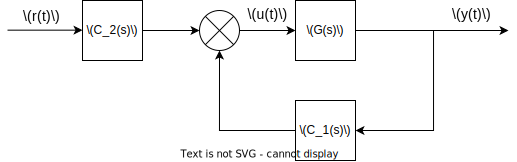
\includegraphics[width=1\linewidth]{./figs/controleIntegral} \caption{Controle integral}\label{fig:unnamed-chunk-45}
\end{figure}

Esse diagrama pode ser modificado para utilizar a estrutura convencional
de controle com realimentação unitária, mas nesse caso, o bloco que
alimenta a referência sofre modificação (\emph{desafio: verifique que
diagrama é esse})

\hypertarget{simulauxe7uxe3o-em-malha-fechada-1}{%
\subsection{Simulação em malha fechada}\label{simulauxe7uxe3o-em-malha-fechada-1}}

Com a realimentação do sistema aumentado, as equações em malha fechada
serão:

\begin{align*}
\dot{\mathbf{x}} &= \mathbf{A}\mathbf{x}-\mathbf{B}\mathbf{K}_a\mathbf{z}\\
\dot{\mathbf{z}} &= (\mathbf{A'}-\mathbf{B'}\mathbf{K}_a-\mathbf{L}_0\mathbf{C}')\mathbf{z}+\mathbf{L}_1\mathbf{C}\mathbf{x}+\mathbf{M}\, r\\
y&= \mathbf{Cx}
\end{align*}

Matrizes de malha fechada:

\begin{align}
\mathbf{A}_{\text{mf}} &= \left[\begin{array}{cc}
    \mathbf{A} & -\mathbf{B}\mathbf{K}_a\\
    \mathbf{L}_1\mathbf{C} & \mathbf{A}'-\mathbf{B}'\mathbf{K}_a-\mathbf{L}_0\mathbf{C}'
\end{array}\right]\\
\mathbf{B}_{\text{mf}} &= \left[\begin{array}{cc}
    \mathbf{0}_{n\times 1} \\ \mathbf{M}
\end{array}\right] = \left[\begin{array}{cc}
    \mathbf{0}_{2n\times 1} \\ 1
\end{array}\right]\\
\mathbf{C}_{\text{mf}} &= \left[\begin{array}{cc}
    \mathbf{C} & \mathbf{0}_{1\times (n+1)}
\end{array}\right]\\
\mathbf{D}_{\text{mf}} &= 0
\end{align}

Perceba que a realimentação de estados é feita através do sinal \(u\). O
sinal \(r\), de referência não deve ser usado para realimentar.

\textbf{Exemplo:}

Construa um compensador com controle integral para o sistema \[
\begin{align}
    G(s) = \frac{10}{(s+1)(s+2)}
\end{align}
\] para que \(\xi = 0.7\) e \(\omega_n=2\).

Sistema: \begin{align}
  \dot{\mathbf{x}} &= \left[\begin{matrix}-3 & 2\\10 & 0\end{matrix}\right]\mathbf{x} + \left[\begin{matrix}0\\1\end{matrix}\right]u\\
  y &= \left[\begin{matrix}1 & 0\end{matrix}\right]\mathbf{x}
\end{align}

Matrizes aumentadas:
\begin{align}
\mathbf{A}_a &= \left[\begin{matrix}-3.0 & 2.0 & 0\\10.0 & 0 & 0\\-1.0 & 0 & 0\end{matrix}\right]\\
\mathbf{B}_a &= \left[\begin{matrix}0\\1\\0\end{matrix}\right]
\end{align}\\

Pólos desejados:
\[
  s = -1.4 \pm j 1.4283
\]
Como o projeto ficou de terceira ordem, precisamos completar com um
pólo. Para não interferir na dominância, vamos alocá-lo com uma
frequência natural 5 vezes maior. Assim, o pólo extra será \(s=-10\).

/Usando as matrizes aumentadas e os pólos difinidos, obtemos os ganhos de realimentação de estados:
\begin{align}
  \mathbf{K}_a = \left[\begin{matrix}11.3 & 9.8 & -20.0\end{matrix}\right]
\end{align}

Para o projeto do observador, podemos usar pólos distantes em um fator de 10 dos pólos originais. Usando o método de Ackerman, obtemos:

\begin{align}
  \mathbf{L} = \left[\begin{matrix}25.0\\210.0\end{matrix}\right]
\end{align}

Para escrever as equações de estado do controlador, calculamos as matrizes em blocos conforme estabelecido:

\begin{align}
  \dot{\mathbf{z}} &= \left[\begin{matrix}-28.0 & 2.0 & 0\\-211.3 & -9.8 & 20.0\\0 & 0 & 0\end{matrix}\right] \mathbf{z} +  \left[\begin{matrix}25.0 & 0\\210.0 & 0\\-1.0 & 1.0\end{matrix}\right] \begin{bmatrix}y \\ r\end{bmatrix}\\
  u &= \left[\begin{matrix}-11.3 & -9.8 & 20.0\end{matrix}\right] \mathbf{z}
\end{align}

\hypertarget{controle-digital}{%
\chapter{Controle Digital}\label{controle-digital}}

No cenário atual onde os computadores digitais estão presentes em todos os aspectos das nossas vidas, não é estranho que microprocessadores sejam usados também em sistemas de controle automático. Neste capítulo vamos estudar de uma forma geral como isso pode ser feito.

\hypertarget{amostras}{%
\section{Amostras}\label{amostras}}

A principal diferença entre o controle analógico com o qual temos trabalhado e o controle digital feito por microprocessadores é que os sinais passam a ser amostrados ou discretos.

Um sinal é discreto quando os únicos valores que importam são aqueles que ocorrem em um instante de tempo específico. Esses instantes denotam um domínio discreto, normalmente são múltiplos inteiros de uma constante real.

Função contínua: \(x(t)=\cos (2\pi t)\). \(t\) pode assumir qualquer valor real.

Função ou sinal discreto: \(x[k] = \cos(0.2\pi k )\). \(k\) só pode assumir valores inteiros. \(k=0\), \(\pm 1\), \(\pm 2\), \(\ldots\).

Essa distinção é necessária porque os computadores digitais trabalham de forma síncrona e discreta: as tarefas só são realizadas em instantes específicos de tempo, que são cronometrados pelo relógio (clock) do processador: na subida ou na descida do clock.

Entre um clock e outro, o computador não executa nenhuma ação e os sinais são ``segurados'' em um valor constante (ou simplesmente consideramos que seja zero).

Graficamente, representamos sinais contínuos por uma linha cheia. Sinais discretos representamos apenas pelos pontos correspondentes às amostras (as linhas verticais são apenas ilustrativas).

\begin{center}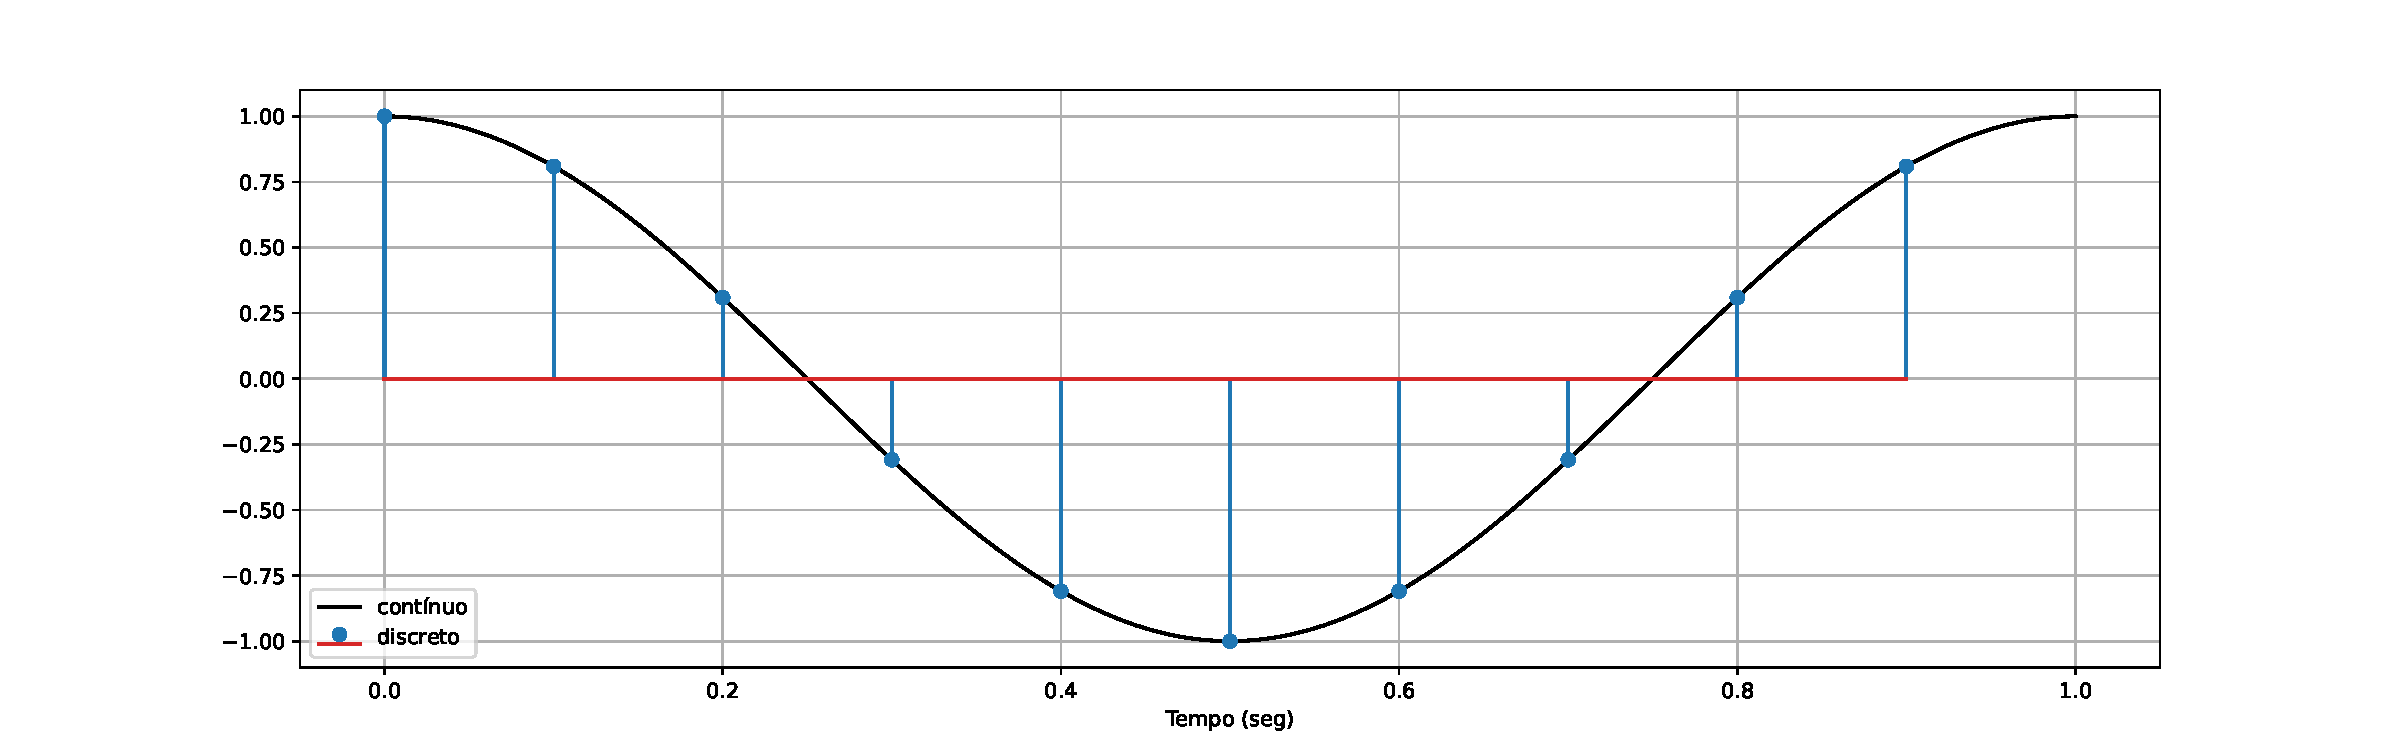
\includegraphics{_main_files/figure-latex/unnamed-chunk-50-1} \end{center}

O gráfico acima representa a função \(\cos(2\pi t)\) contínua e discretizada. A linha preta cheia é o sinal analógico. Ele existe para qualquer instante de tempo, por exemplo \(t=\sqrt{2}\), \(t=1/9\). A função denotada por pontos circulares azuis é a versão discreta da mesma função. Observe que os valores do eixo Y são os mesmos do sinal analógico. Porém, as linhas azuis só ocorrem nos instantes \(0.1\), \(0.2\), etc. Todos são múltiplos inteiros de \(0.1\) segundos.

Um sinal discreto é muito mais simples de representar no computador. Basta armazenar as amostras em um vetor. O sinal representado acima foi gerado em Python e consiste das seguintes amostras.

\hypertarget{conversor-ad}{%
\section{Conversor A/D}\label{conversor-ad}}

O conversor Analógico-Digital (A/D) é um elemento conceitual que converte um sinal contínuo no tempo para um sinal discreto no tempo.

Na prática ele é implementado como um circuito de chaveamento: a chave fecha para coletar o sinal e abre até que o próximo clock mande coletar outra amostra.

Existe uma \href{https://dewesoft.com/daq/types-of-adc-converters}{variedade} grande de conversores A/D. A maioria está disponível em um chip eletrônico convencional que pode ser controlado por um microprocessador. Contudo, o mais comum é despachar o microprocessador e o conversor A/D em um único chip, que na prática é o que chamamos de microcontrolador.

Nosso escopo aqui não é discutir os circuitos de conversão, isso fica para as aulas de eletrônica. No entanto, precisamos entender os efeitos dele no sistema de controle.

O principal efeito é a discretização do sinal, o que produz atraso na malha de controle.

Outro efeito secundário é a introdução de erro na medição, porque a representação digital sempre arredonda valores para que o computador possa fazer as contas. Essa é a discretização de amplitude. Você deve ter aprendido isso em Eletrônica Digital. Ela também é importante, mas neste curso não vamos analisar seus efeitos, porque a maioria dos conversores usam uma resolução elevada (10 bits, pelo menos) e isso normalmente é mais que suficiente para desprezarmos os efeitos na maioria dos processos de controle realimentado.

\hypertarget{peruxedodo-de-amostragem}{%
\section{Período de amostragem}\label{peruxedodo-de-amostragem}}

É o menor intervalo de tempo entre uma amostra e outra, supondo que elas sejam coletadas sempre no mesmo intervalo.

O inverso do período de amostragem é chamado de \emph{taxa de amostragem} é medida em amostras por segundo, ou ciclos por segundo, cuja unidade típica é Hertz.

\[
\begin{align}
    f = \frac{1}{T}\quad\quad \text{(Hertz)}
\end{align}
\]

Um sistema que coleta uma amostra de um sinal a cada \(0.001\) segundos possui período de amostragem de \(1\) milissegundo e uma taxa de amostragem de 1 kilo Hertz.

Existem sistemas de conversão A/D que trabalham com período de amostragem variável, mas não será o caso que vamos estudar neste curso.

Quanto menor o período de amostragem ``mais fiel'' o sinal amostrado será ao sinal contínuo (isso depende da resolução também). No entanto, quando mais ``rápida'' essa amostragem é, mais caro o conversor fica, tando economicamente (chips mais rápidos custam mais dinheiro) quanto do ponto de vista de energia, pois circuitos que chaveiam muito esquentam demais.

\begin{Shaded}
\begin{Highlighting}[]
\ImportTok{import}\NormalTok{ numpy }\ImportTok{as}\NormalTok{ np}
\ImportTok{import}\NormalTok{ matplotlib.pyplot }\ImportTok{as}\NormalTok{ plt}
\NormalTok{t }\OperatorTok{=}\NormalTok{ np.linspace(}\DecValTok{0}\NormalTok{,}\DecValTok{1}\NormalTok{,}\DecValTok{100}\NormalTok{)}
\NormalTok{x }\OperatorTok{=}\NormalTok{ np.cos(}\DecValTok{2}\OperatorTok{*}\NormalTok{np.pi}\OperatorTok{*}\NormalTok{t)}
\NormalTok{T1 }\OperatorTok{=} \FloatTok{0.1}
\NormalTok{k1 }\OperatorTok{=}\NormalTok{ np.arange(}\DecValTok{10}\NormalTok{)}
\NormalTok{xs1 }\OperatorTok{=}\NormalTok{ np.cos(}\DecValTok{2}\OperatorTok{*}\NormalTok{np.pi}\OperatorTok{*}\NormalTok{k1}\OperatorTok{*}\NormalTok{T1)}
\NormalTok{T2 }\OperatorTok{=} \FloatTok{0.02}
\NormalTok{k2 }\OperatorTok{=}\NormalTok{ np.arange(}\BuiltInTok{int}\NormalTok{(}\DecValTok{1}\OperatorTok{/}\NormalTok{T2))}
\NormalTok{xs2 }\OperatorTok{=}\NormalTok{ np.cos(}\DecValTok{2}\OperatorTok{*}\NormalTok{np.pi}\OperatorTok{*}\NormalTok{k2}\OperatorTok{*}\NormalTok{T2)}
\NormalTok{plt.figure(figsize}\OperatorTok{=}\NormalTok{(}\DecValTok{16}\NormalTok{,}\DecValTok{5}\NormalTok{))}
\NormalTok{plt.plot(t,x,}\StringTok{\textquotesingle{}k\textquotesingle{}}\NormalTok{,label}\OperatorTok{=}\StringTok{\textquotesingle{}contínuo\textquotesingle{}}\NormalTok{)}
\NormalTok{plt.step(k1}\OperatorTok{*}\NormalTok{T1,xs1,label}\OperatorTok{=}\SpecialStringTok{f\textquotesingle{}T=}\SpecialCharTok{\{}\NormalTok{T1}\SpecialCharTok{\}}\SpecialStringTok{\textquotesingle{}}\NormalTok{)}
\NormalTok{plt.step(k2}\OperatorTok{*}\NormalTok{T2,xs2,label}\OperatorTok{=}\SpecialStringTok{f\textquotesingle{}T=}\SpecialCharTok{\{}\NormalTok{T2}\SpecialCharTok{\}}\SpecialStringTok{\textquotesingle{}}\NormalTok{)}
\NormalTok{plt.xlabel(}\StringTok{\textquotesingle{}Tempo (seg)\textquotesingle{}}\NormalTok{)}
\NormalTok{plt.legend()}
\NormalTok{plt.show()}
\end{Highlighting}
\end{Shaded}

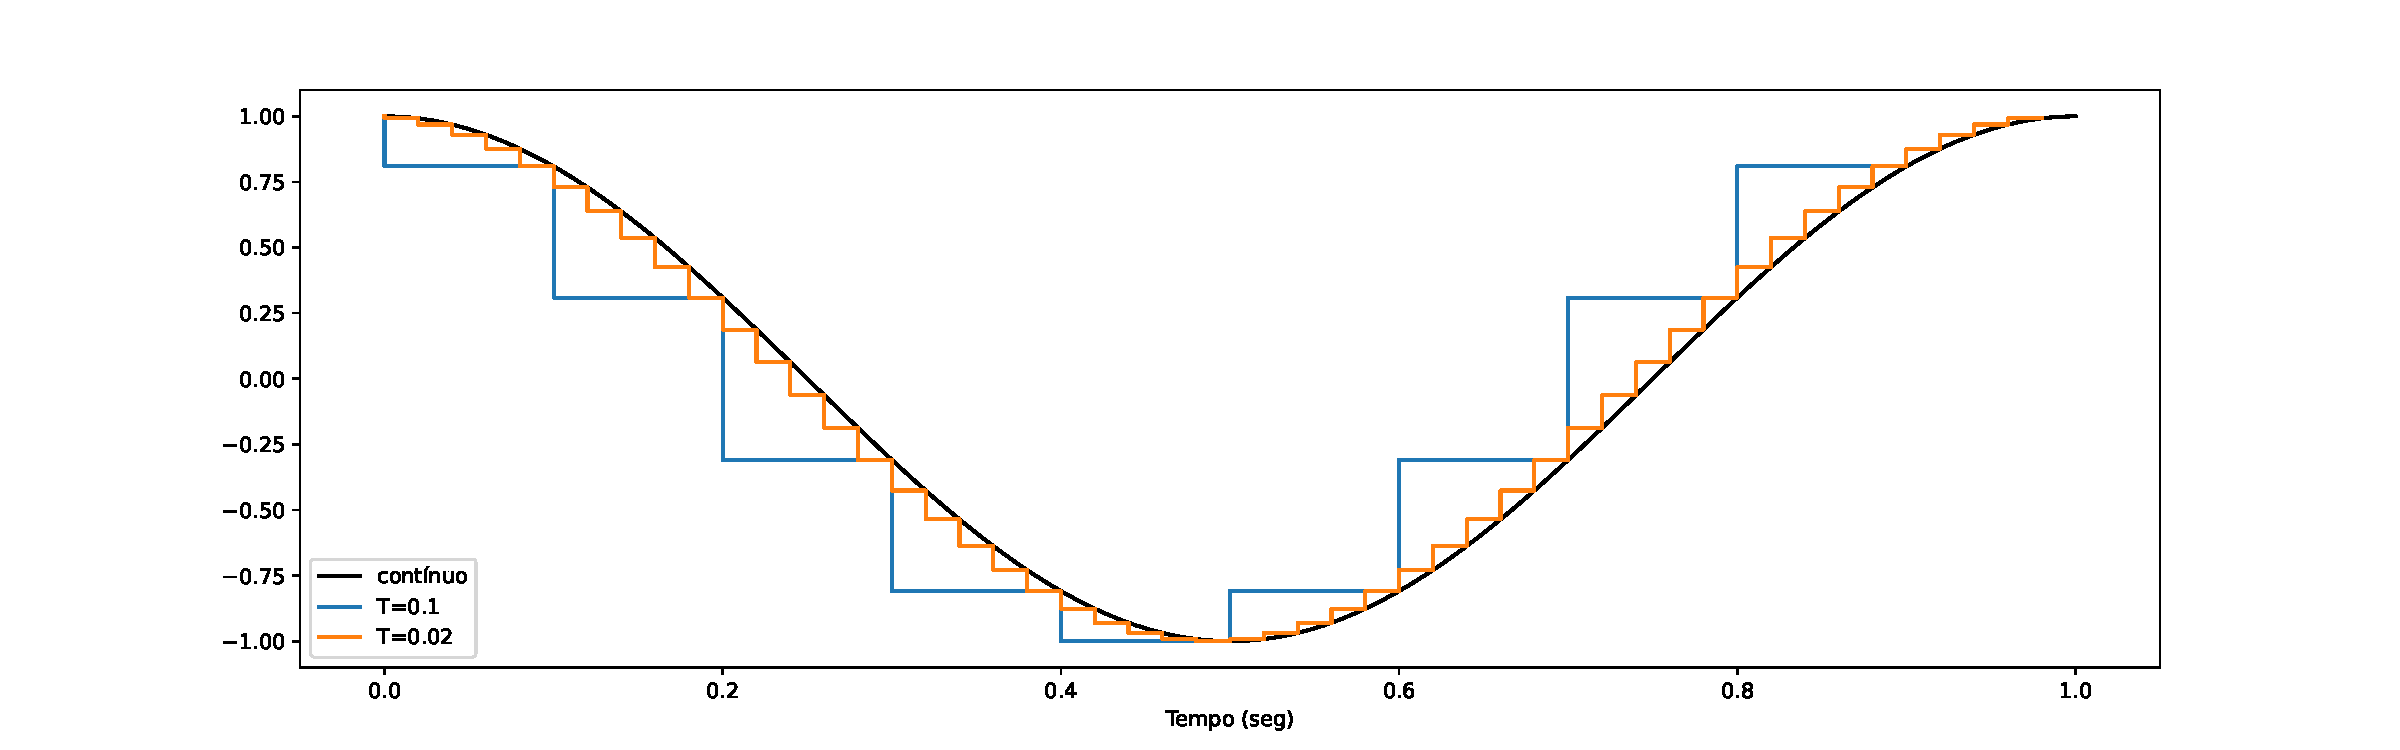
\includegraphics{_main_files/figure-latex/unnamed-chunk-51-3.pdf}

Note que o período de amostragem não é necessariamente o clock do processador, porque às vezes o processador trabalha mais rápido do que o nosso sistema precisa. Por exemplo, sistemas de temperatura normalmente são lentos, e não é raro eles terem período de amostagem de 1 ou mais segundos. Para um Arduino, entretanto, cujo clock é 16 MHz, 1 segundo equivale a vários clocks. Tudo isso é controlável pelo projetista.

Para ``baratear'' nosso sistema, então, podemos escolher processadores mais lentos. Mas ele não pode haver exagero. Se ele for lento demais, o conversor A/D não conseguirá ``perceber'' as mudanças significativas do sinal, ou seja, informação será perdida. Se não tivermos informação, o controle não tem como funcionar.

Há um critério matemático que estabelece qual a mínima taxa de amostragem que devemos usar para uma dada situação; é o teorema da amostragem de Shannon-Nyquist. Vamos discutí-lo posteriormente.

\hypertarget{sistemas-de-controle-digital}{%
\section{Sistemas de controle digital}\label{sistemas-de-controle-digital}}

A figura 8.1 mostra como funciona conceitualmente um sistema de controle digital, em relação a um sistema equivalente analógico.

O que está acontecendo?

\begin{itemize}
\tightlist
\item
  O sinal analógico do sensor \(y(t)\) é convertido em um sinal discreto \(y(kT)\), através do amostrador e do circuito A/D
\item
  O sinal de referência é agora um sinal discreto \(r(kT)\), gerado dentro do controlador digital.
\item
  O sinal de controle \(u(kT)\) é calculado no programa do controlador através de uma equação de diferenças, e não mais por um circuito analógico
\item
  O sinal de controle \(u(kT)\) é convertido para um sinal analógico \(u(t)\) pelo conversor D/A + segurador, antes de ir de volta para a planta.
\end{itemize}

A principal desvantagem do controle digital é o atraso nos sinais devido ao procedimento de amostragem e conversão.

A informação entre uma amostra e outra é perdida. Essa perda faz com que o controle trabalhe sempre com uma informação atrasada. Se o controlador digital fosse um circuito analógico, esse atraso seria equivalente a uma perda pura de tempo de aproximadamente \(T/2\)

  \bibliography{book.bib,packages.bib}

\end{document}
